\documentclass[12pt,oneside,a4paper]{book}
\usepackage{fullpage}
%\usepackage[toc,page]{appendix}

\usepackage{caption}
\usepackage{subcaption}
\usepackage{amsmath}
\usepackage{amsthm}

% Quotes
\usepackage{upquote}

% Code listing setup
\usepackage{listings}
\usepackage{color} %need to use color to define those colors below
\definecolor{codegreen}{rgb}{0,0.6,0}
\definecolor{codegray}{rgb}{0.5,0.5,0.5}
\definecolor{codepurple}{rgb}{0.58,0,0.82}
\definecolor{backcolour}{rgb}{0.95,0.95,0.92}
\lstset{
    commentstyle=\color{red},
    keywordstyle=\color{blue},
    backgroundcolor=\color{backcolour},   
    commentstyle=\color{codegreen},
    keywordstyle=\color{magenta},
    numberstyle=\tiny\color{codegray},
    stringstyle=\color{codepurple},
    literate={~} {$\sim$}{1},
    escapechar=£,
    basicstyle=\scriptsize,
    frame=single,
    showstringspaces=false,
    breaklines,
    language=Octave,
}
% Rermove indent in list of listing
\makeatletter
\renewcommand*{\l@lstlisting}{\@dottedtocline{1}{0em}{2.3em}}
\makeatother


% Hyper link setup
\usepackage{hyperref}
\hypersetup
{
    colorlinks=true,
    linkcolor=blue,
    urlcolor=red,
    linktoc=all
}

% Graphicx setup
\usepackage{graphicx}
\graphicspath{ {images/} }

% No indent at the first line of a paragraph
\setlength\parindent{0pt}

% List of equations
\usepackage[titles]{tocloft}
\newcommand{\listequationsname}{List of Equations}
\newlistof{myequations}{equ}{\listequationsname}
% myequation takes in its display name
\newcommand{\myequations}[1]{%
% display name is printed
%\addcontentsline{equ}{myequations}{\protect\numberline{\theequation}#1}\par}
\addcontentsline{equ}{myequations}{\protect\numberline{\theequation}#1}}
\setlength{\cftmyequationsnumwidth}{2.3em}% Width of equation number in List of Equations

% List of alignment
\newcommand{\listalignsname}{List of Formulas}
\newlistof{myaligns}{ali}{\listalignsname}
% myaligns takes in its display name
\newcommand{\myaligns}[1]{%
% display name is printed
\addcontentsline{ali}{myaligns}{\protect\numberline{\theequation}#1}}
\setlength{\cftmyalignsnumwidth}{2.3em}% Width of formula number in List of Formulas

\setlength{\cftfigindent}{0pt}  % remove indentation from figures in lof
\setlength{\cfttabindent}{0pt}  % remove indentation from tables in lot


% INDICES: NOT SO USEFUL IN MY CASE
% \usepackage{imakeidx}
% \makeindex[columns=2, title=Alphabetical Index, intoc]

% To use mathbb represents mathematical form of capital letters
\usepackage{amsfonts} 

%% ---------------------------- BEGIN DOCUMENT ----------------------------

\begin{document}
\boldmath
\begin{titlepage}
    \begin{center}
        %\vspace*{1cm}
        
        \Huge
        \textbf{Course Note}
        
        \vspace{0.5cm}
        \LARGE
        Machine Learning by Prof. Andrew Ng
        
        \vspace{1.5cm}
        
        \textbf{Hong Anh VU}\\
        vuhonganh91 at gmail dot com\\
        March 2016
        
        \vfill        

        \begin{figure}[!ht]
          \centering
          
\includegraphics[scale=0.28]{xLogo.eps}
        \end{figure}
        
        \Large
        Ecole Polytechnique\\
        Promotion X2011\\
        
    \end{center}
\end{titlepage}

%\setcounter{tocdepth}{2}
\tableofcontents

% \makeatletter
% \def\@@underline#1{#1}
% \tableofcontents
% \makeatother


\listoffigures

\lstlistoflistings

%\listofmyequations %use myaligns instead

\listofmyaligns

\chapter{Week 1} 
This is the week 1 of the course Probabilistic Graphical Models (pgm) by Prof. Daphne Koller hosted on Coursera. The week 1 covers quite a lot of notions from distribution to Bayesian Network.

\section{Distribution}
A probability distribution function (aka PDF, probability density function, probability function, or density) is a function that indicates the probability that a given random variable will take on a particular value. If a random variable is discrete (i.e. the value of the random variable is contained in a countable set of values), then the probability density function, $f(x)$ of a random variable $X$ is: $f(x) = P(X = x)$.

The multivariate form of a probability distribution function is the probability that a list of random variables will take on a list of values. If the random variables are discrete, the \textbf{joint probability density function}, $f(x_1, x_2, …, x_n)$ for random variables $X_1, X_2, ..., X_n$ is defined by: 
\begin{align}
f(x_1, x_2, \ldots, x_n) = P(X_1=x_1, X_2=x_2, \ldots, X_n=x_n)
\end{align}
\myaligns{Joint Distribution}

\section{Factors}
A factor is a function or a table or a mapping from every assignment of arguments to a real value. We define below factor $\Phi(X_1, \ldots, X_k)$ where $(X_1, \ldots, X_k)$ which is the scope (a set of random variables).
\begin{align}
\Phi: Val(X_1, \ldots, X_k) \rightarrow \mathbb{R}
\end{align}
\myaligns{Factor Definition}

\subsection{Examples of Factor}
Hence, according to the definition above, a joint distribution is a factor. Figure \ref{w1JointDistri} illustrates a joint distribution $P(I,D,G)$ where $I$, $D$, $G$ represents intelligence of a student $(0, 1)$, difficulty of a course $(0,1)$, and the final grade $(A,B,C)$ that student got from that course respectively.
\begin{figure}[!ht]
\centering
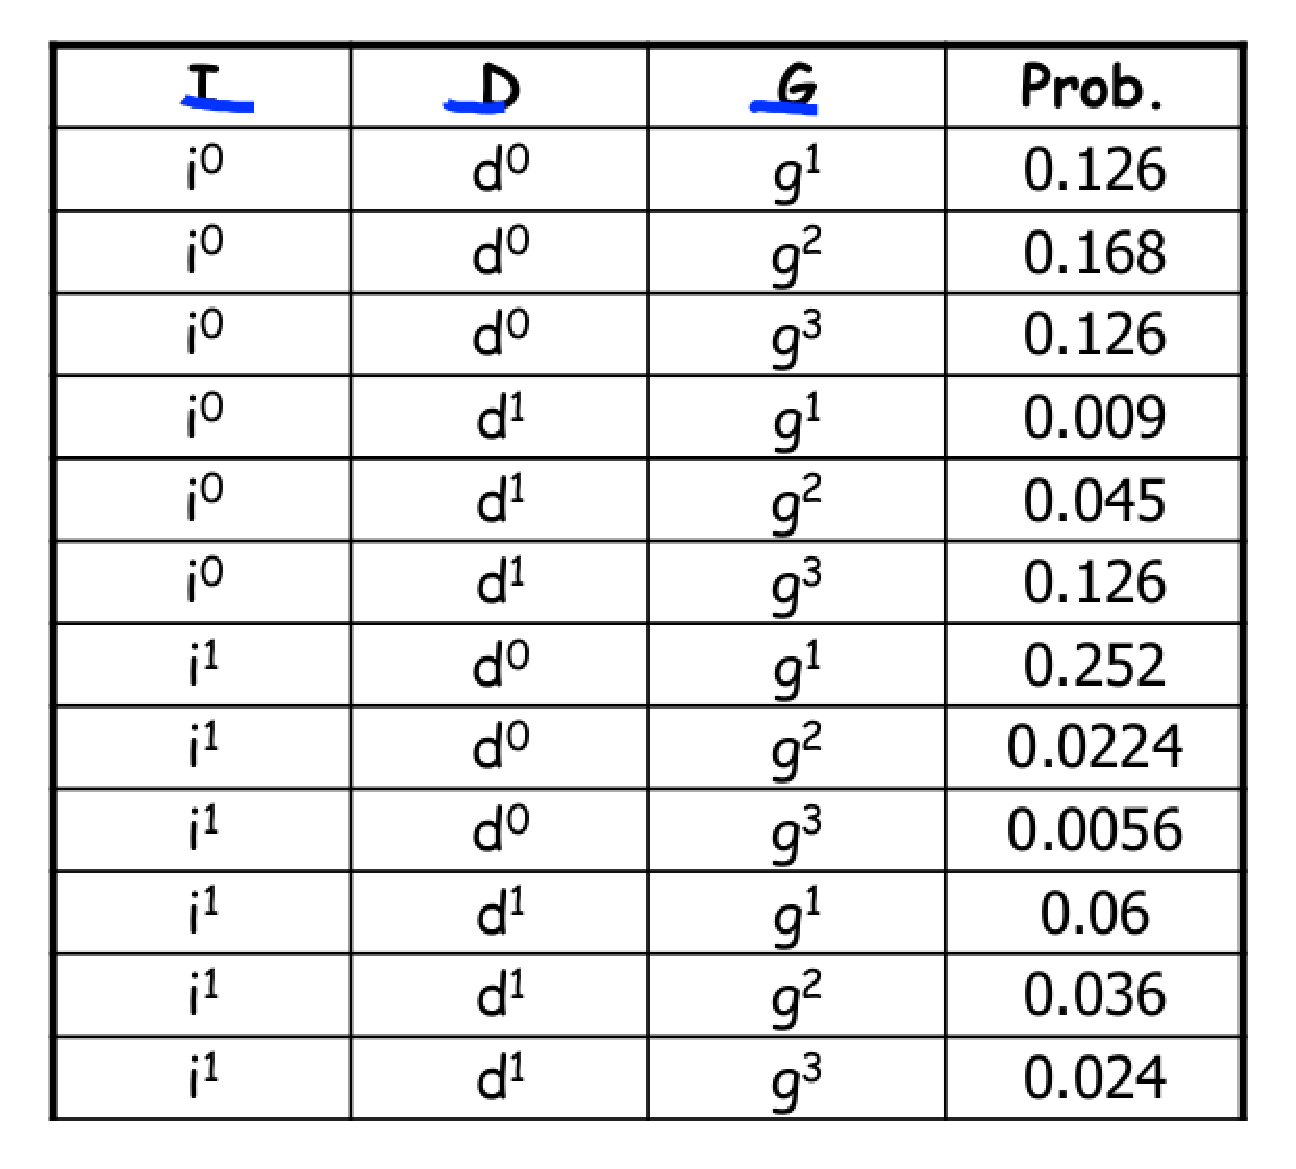
\includegraphics[scale = 0.3]{w1JointDistri}
\caption{Joint Distribution}
\label{w1JointDistri}
\end{figure}

Another example is UnnormaliCed Measure $P(I,D,g^1)$ which has scope $(I,D)$ because $G$ is always fixed to $g^1$. Another \textbf{important example} is Conditional Probability Distribution (CPD). Figure \ref{w1CPD} illustrates the \textbf{CPD} $P(G | I, D)$ which means for every combination of values to the variable $I$ and $D$, we have a probability distribution over $G$.  

\begin{figure}[!ht]
\centering
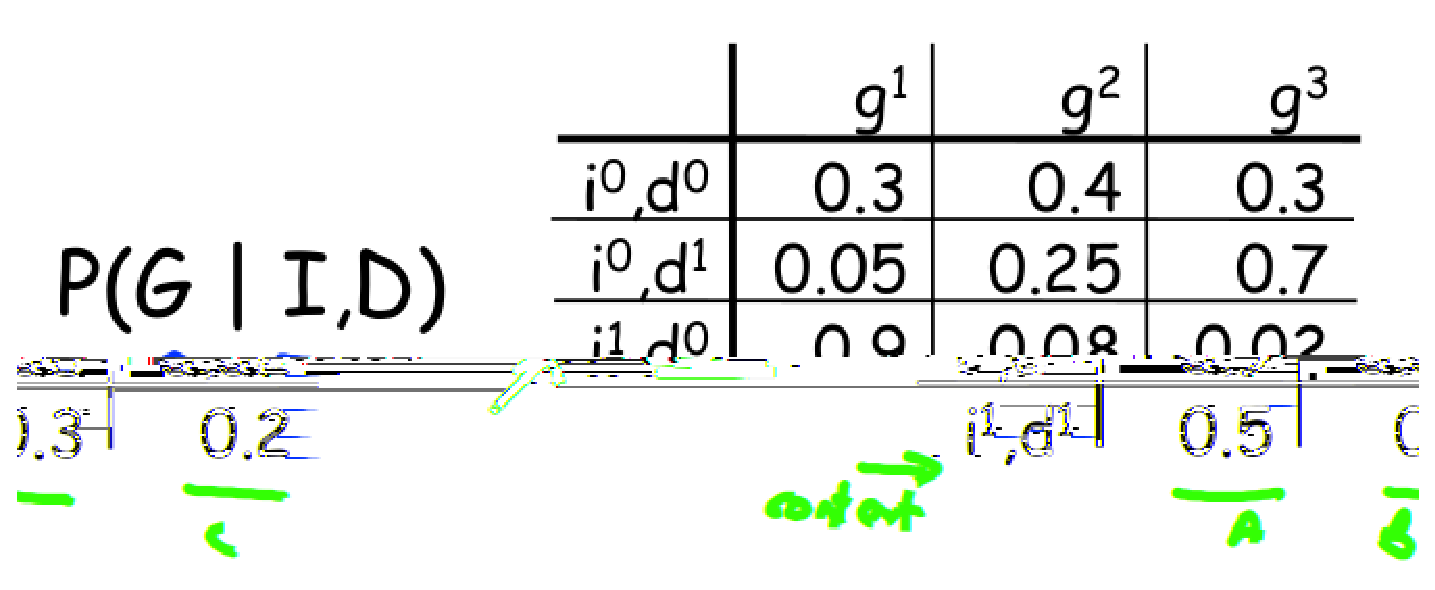
\includegraphics[scale = 0.4]{w1CPD}
\caption{Conditional Probability Distribution (CPD)}
\label{w1CPD}
\end{figure}

\section{Operations on Factors}
\subsection{Factor Products}
If $\Phi_1(A,B)$ and $\Phi_2(B,C)$ are two factors then we compute their product of $\Phi(A,B,C)$ by multiplying $\Phi_1(A,B)\Phi_2(B,C)$ for all common values of $B$ (see figure \ref{w1FactProd}).

\begin{figure}[!ht]
\centering
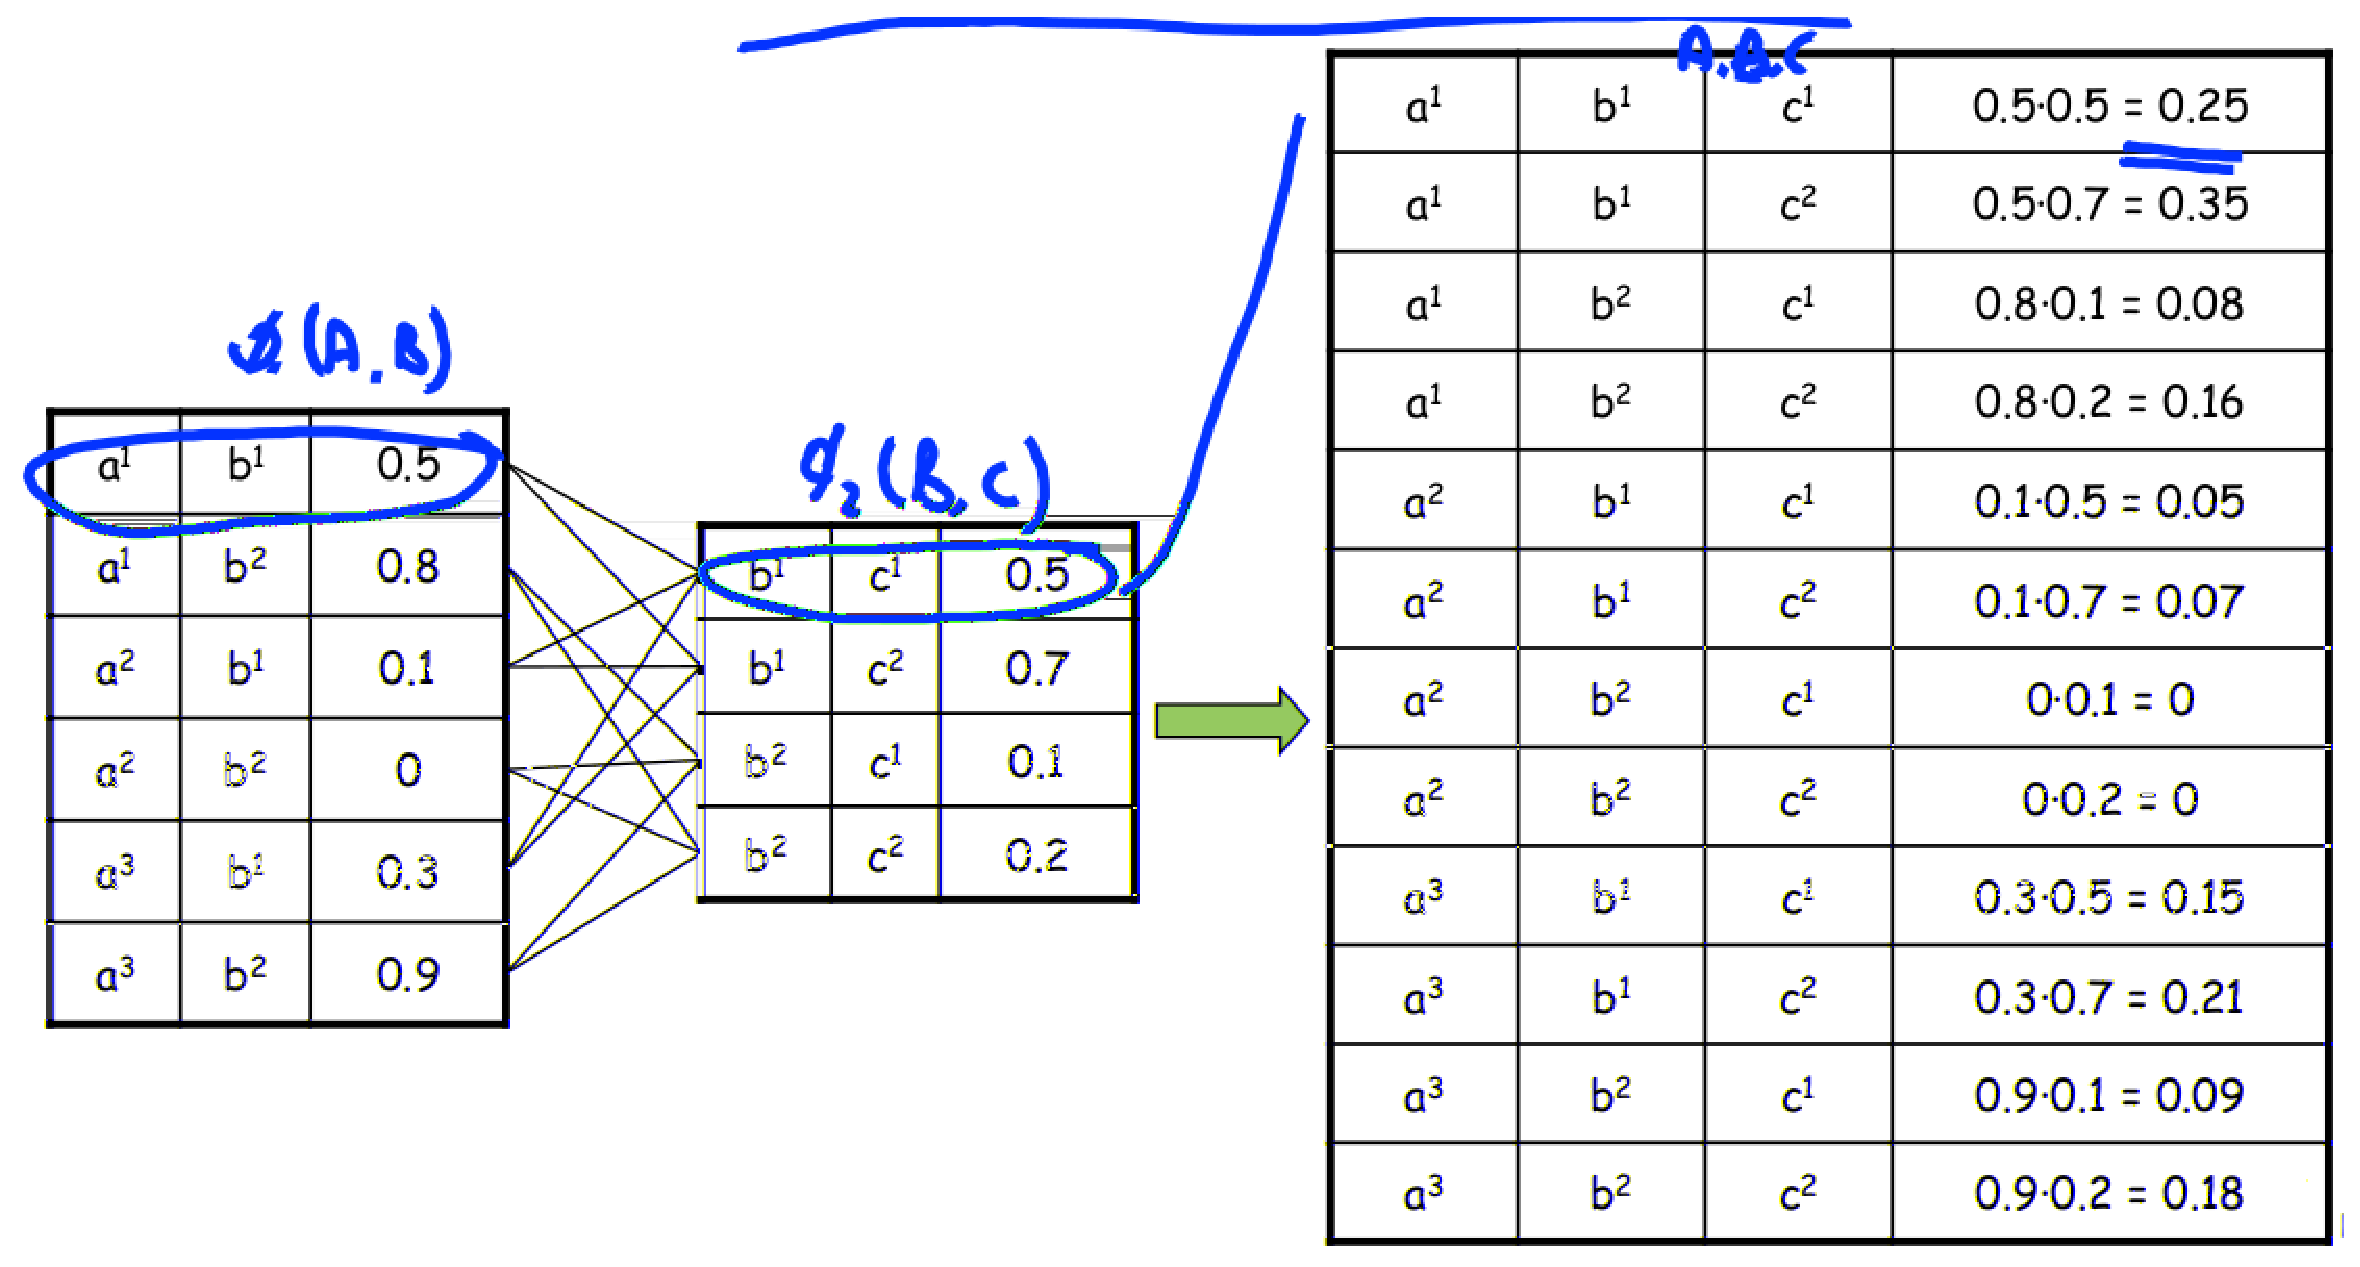
\includegraphics[scale = 0.3]{w1FactProd}
\caption{Factor Products}
\label{w1FactProd}
\end{figure}

\subsection{Factor Marginalization}
That's when we want to reduce the scope. For example, we reduce scope $(A,B,C)$ to $(A,C)$ by summing over $B$ for every assignment of $(A,C)$ (figure \ref{w1FactMarginal}).

\begin{figure}[!ht]
\centering
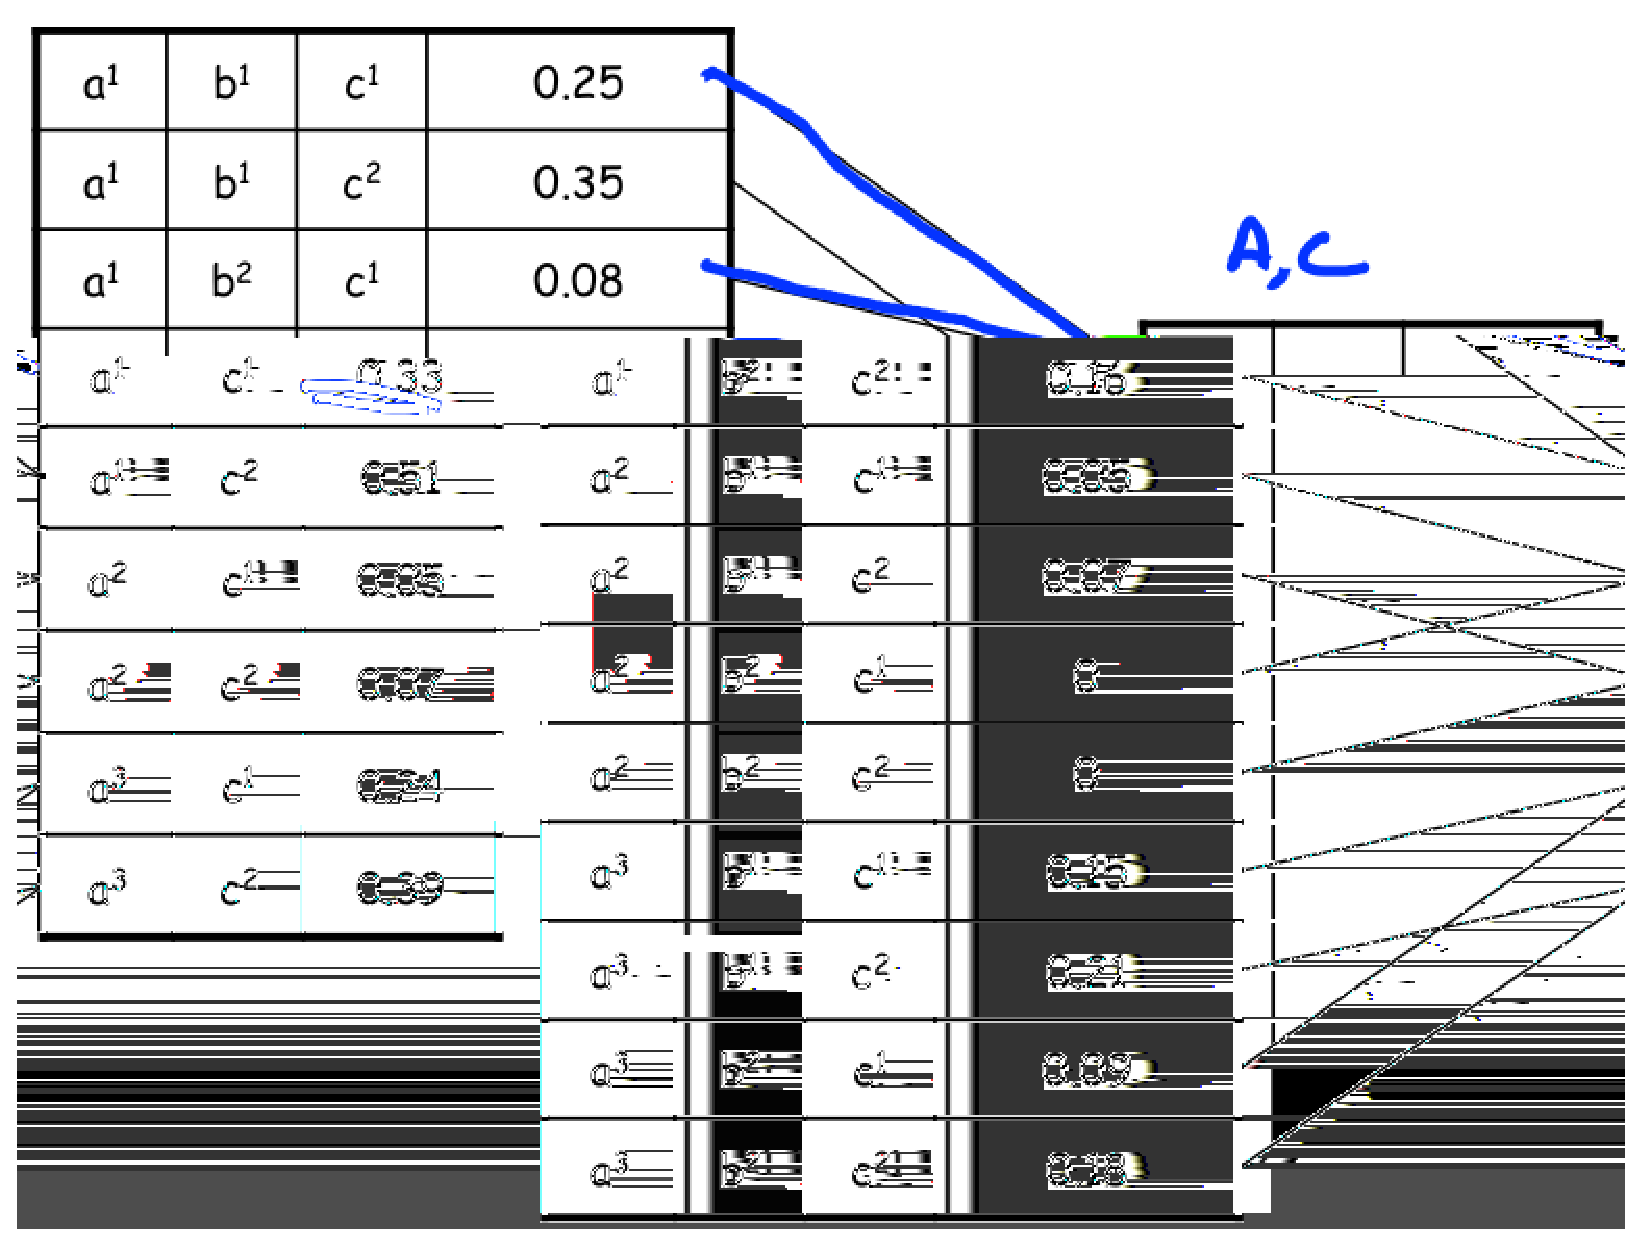
\includegraphics[scale = 0.35]{w1FactMarginal}
\caption{Factor Marginalization}
\label{w1FactMarginal}
\end{figure}

\subsection{Factor Reduction}
That's when we fix a random variable in the scope by one value (in its set of values). For example, $\Phi(A,B,C)$ is reduced to $\Phi(A,B | C = c^1)$ in illustration \ref{w1FactReduce}.
\begin{figure}[!ht]
\centering
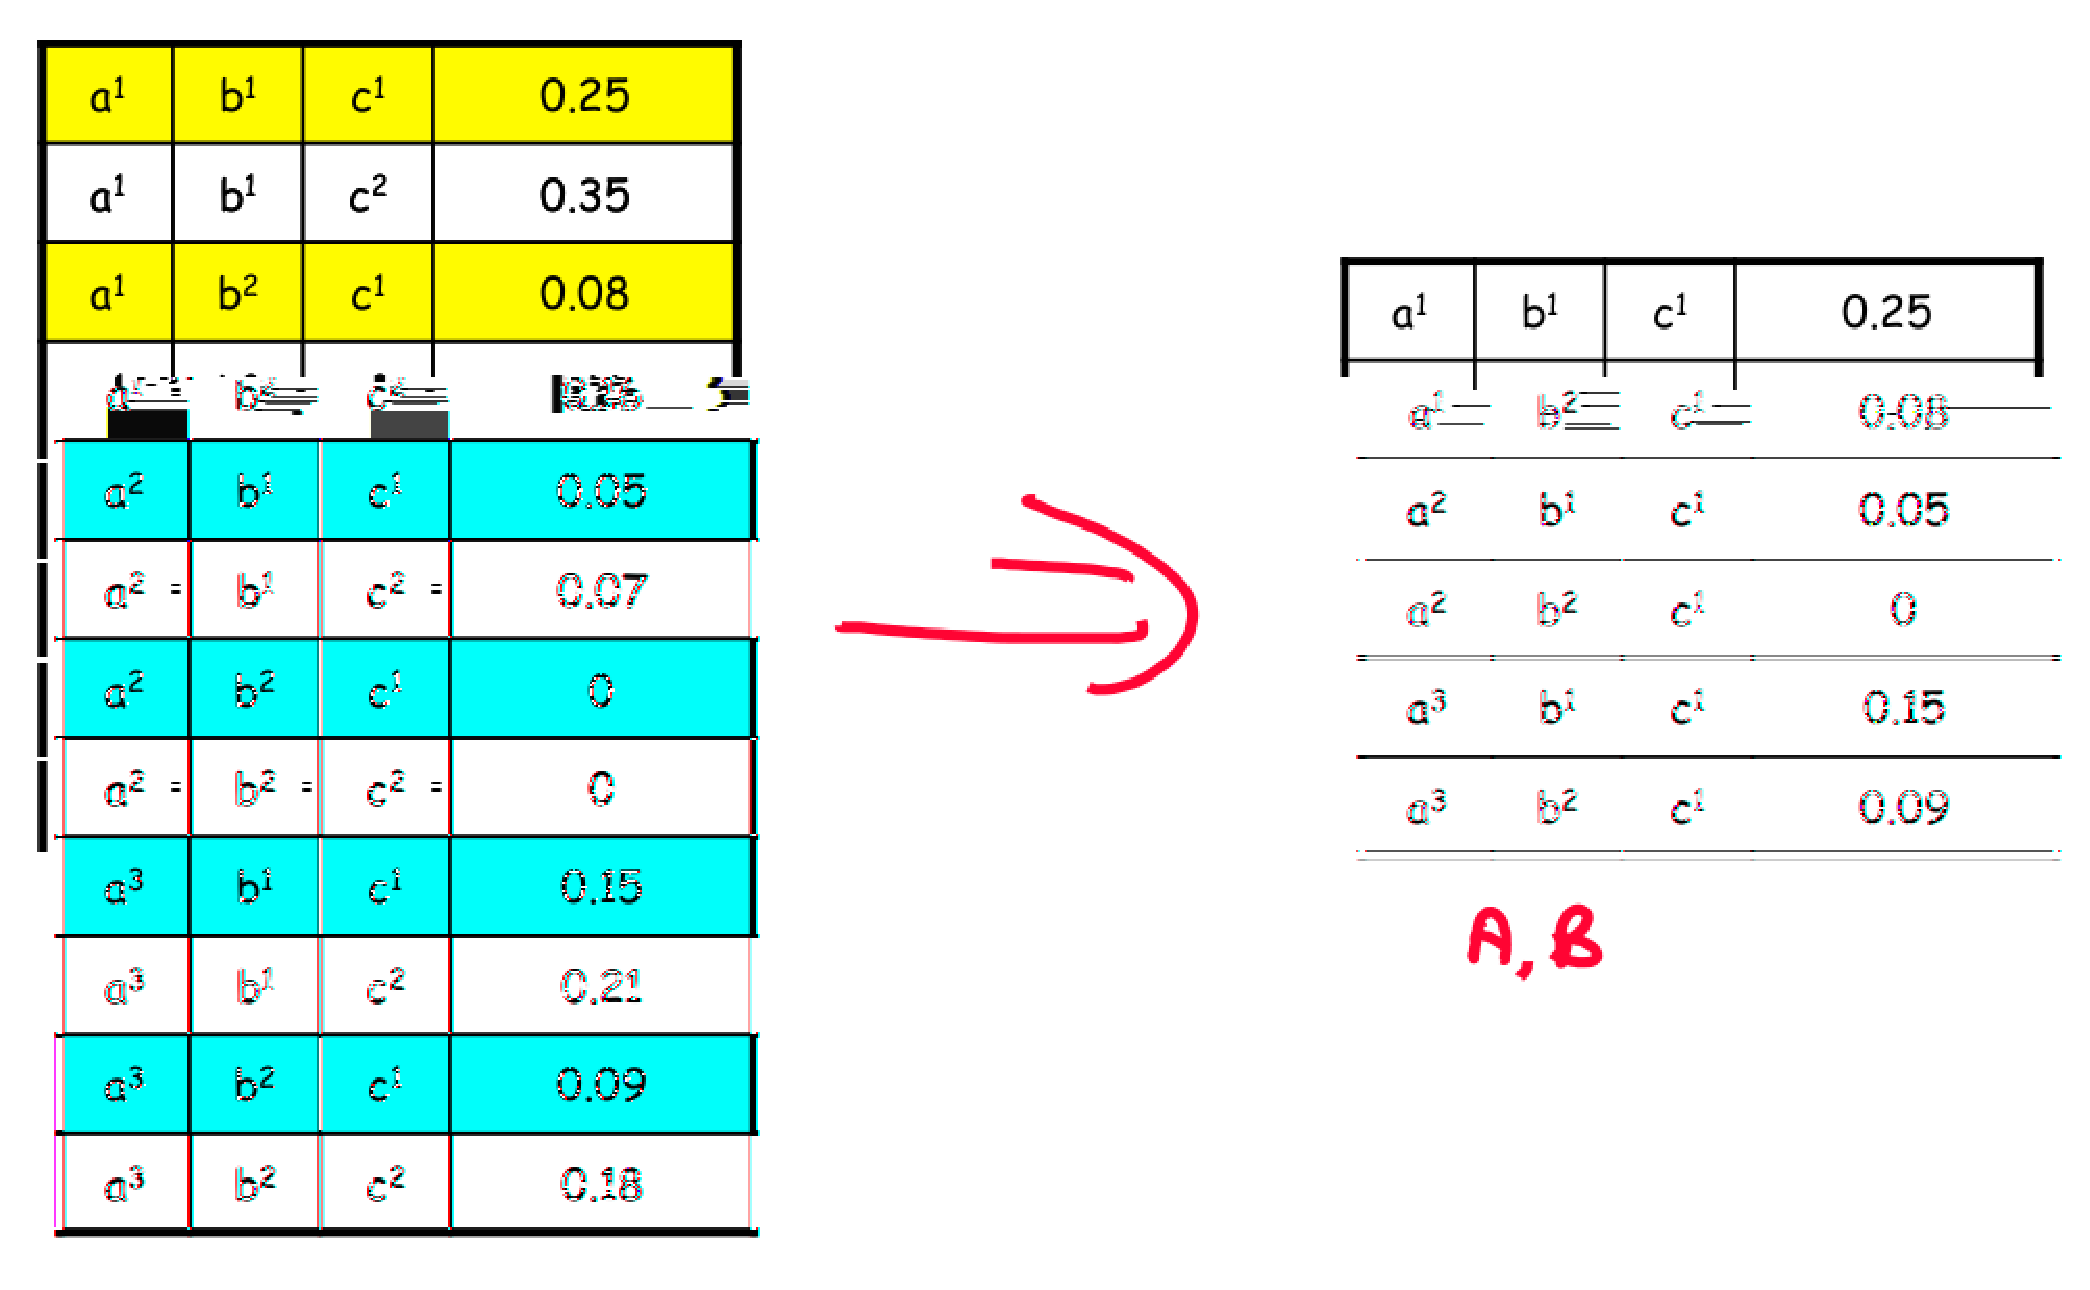
\includegraphics[scale = 0.35]{w1FactReduce}
\caption{Factor Reduction}
\label{w1FactReduce}
\end{figure}

\section{Semantics And Factorization}
\subsection{The Student Example}
The student example involving the situation where students take a course. It contains the following random variables:
\begin{itemize}
	\item Course \textbf{D}ifficulty $(D)$ ($0$ = not difficult, $1$ = difficult)
	\item Student \textbf{I}ntelligence $(I)$ ($0$ = not intelligent, $1$ = intelligent)
	\item \textbf{G}rade $(G)$ ($1$ = A, $2$ = B, $3$ = C)
	\item Student \textbf{S}AT score $(S)$ ($0$ = not good, $1$ = good)
	\item Reference \textbf{L}etter from the prof. of this course $(L)$ ($0$ = not referred, $1$ = referred)
\end{itemize}

The dependency graph is shown in figure \ref{w1graphCPD}. Intuitively, we can see the directed edge meaning a strong relation between the 2 variables. We also annotate each node of the dependency graph to a CPD (Conditional Probability Distribution). NB: I do not know where this comes from, maybe we can calculate them from the data set. We have the chain rule for Bayesian Networks in this example is described in formula below.
\begin{align}
P(G|I,D)P(S|I)P(L|G)P(D)P(I) = P(D,I,G,S,L)
\end{align}
\myaligns{Chain Rule for Bayesian Networks}

\begin{figure}[!ht]
\centering
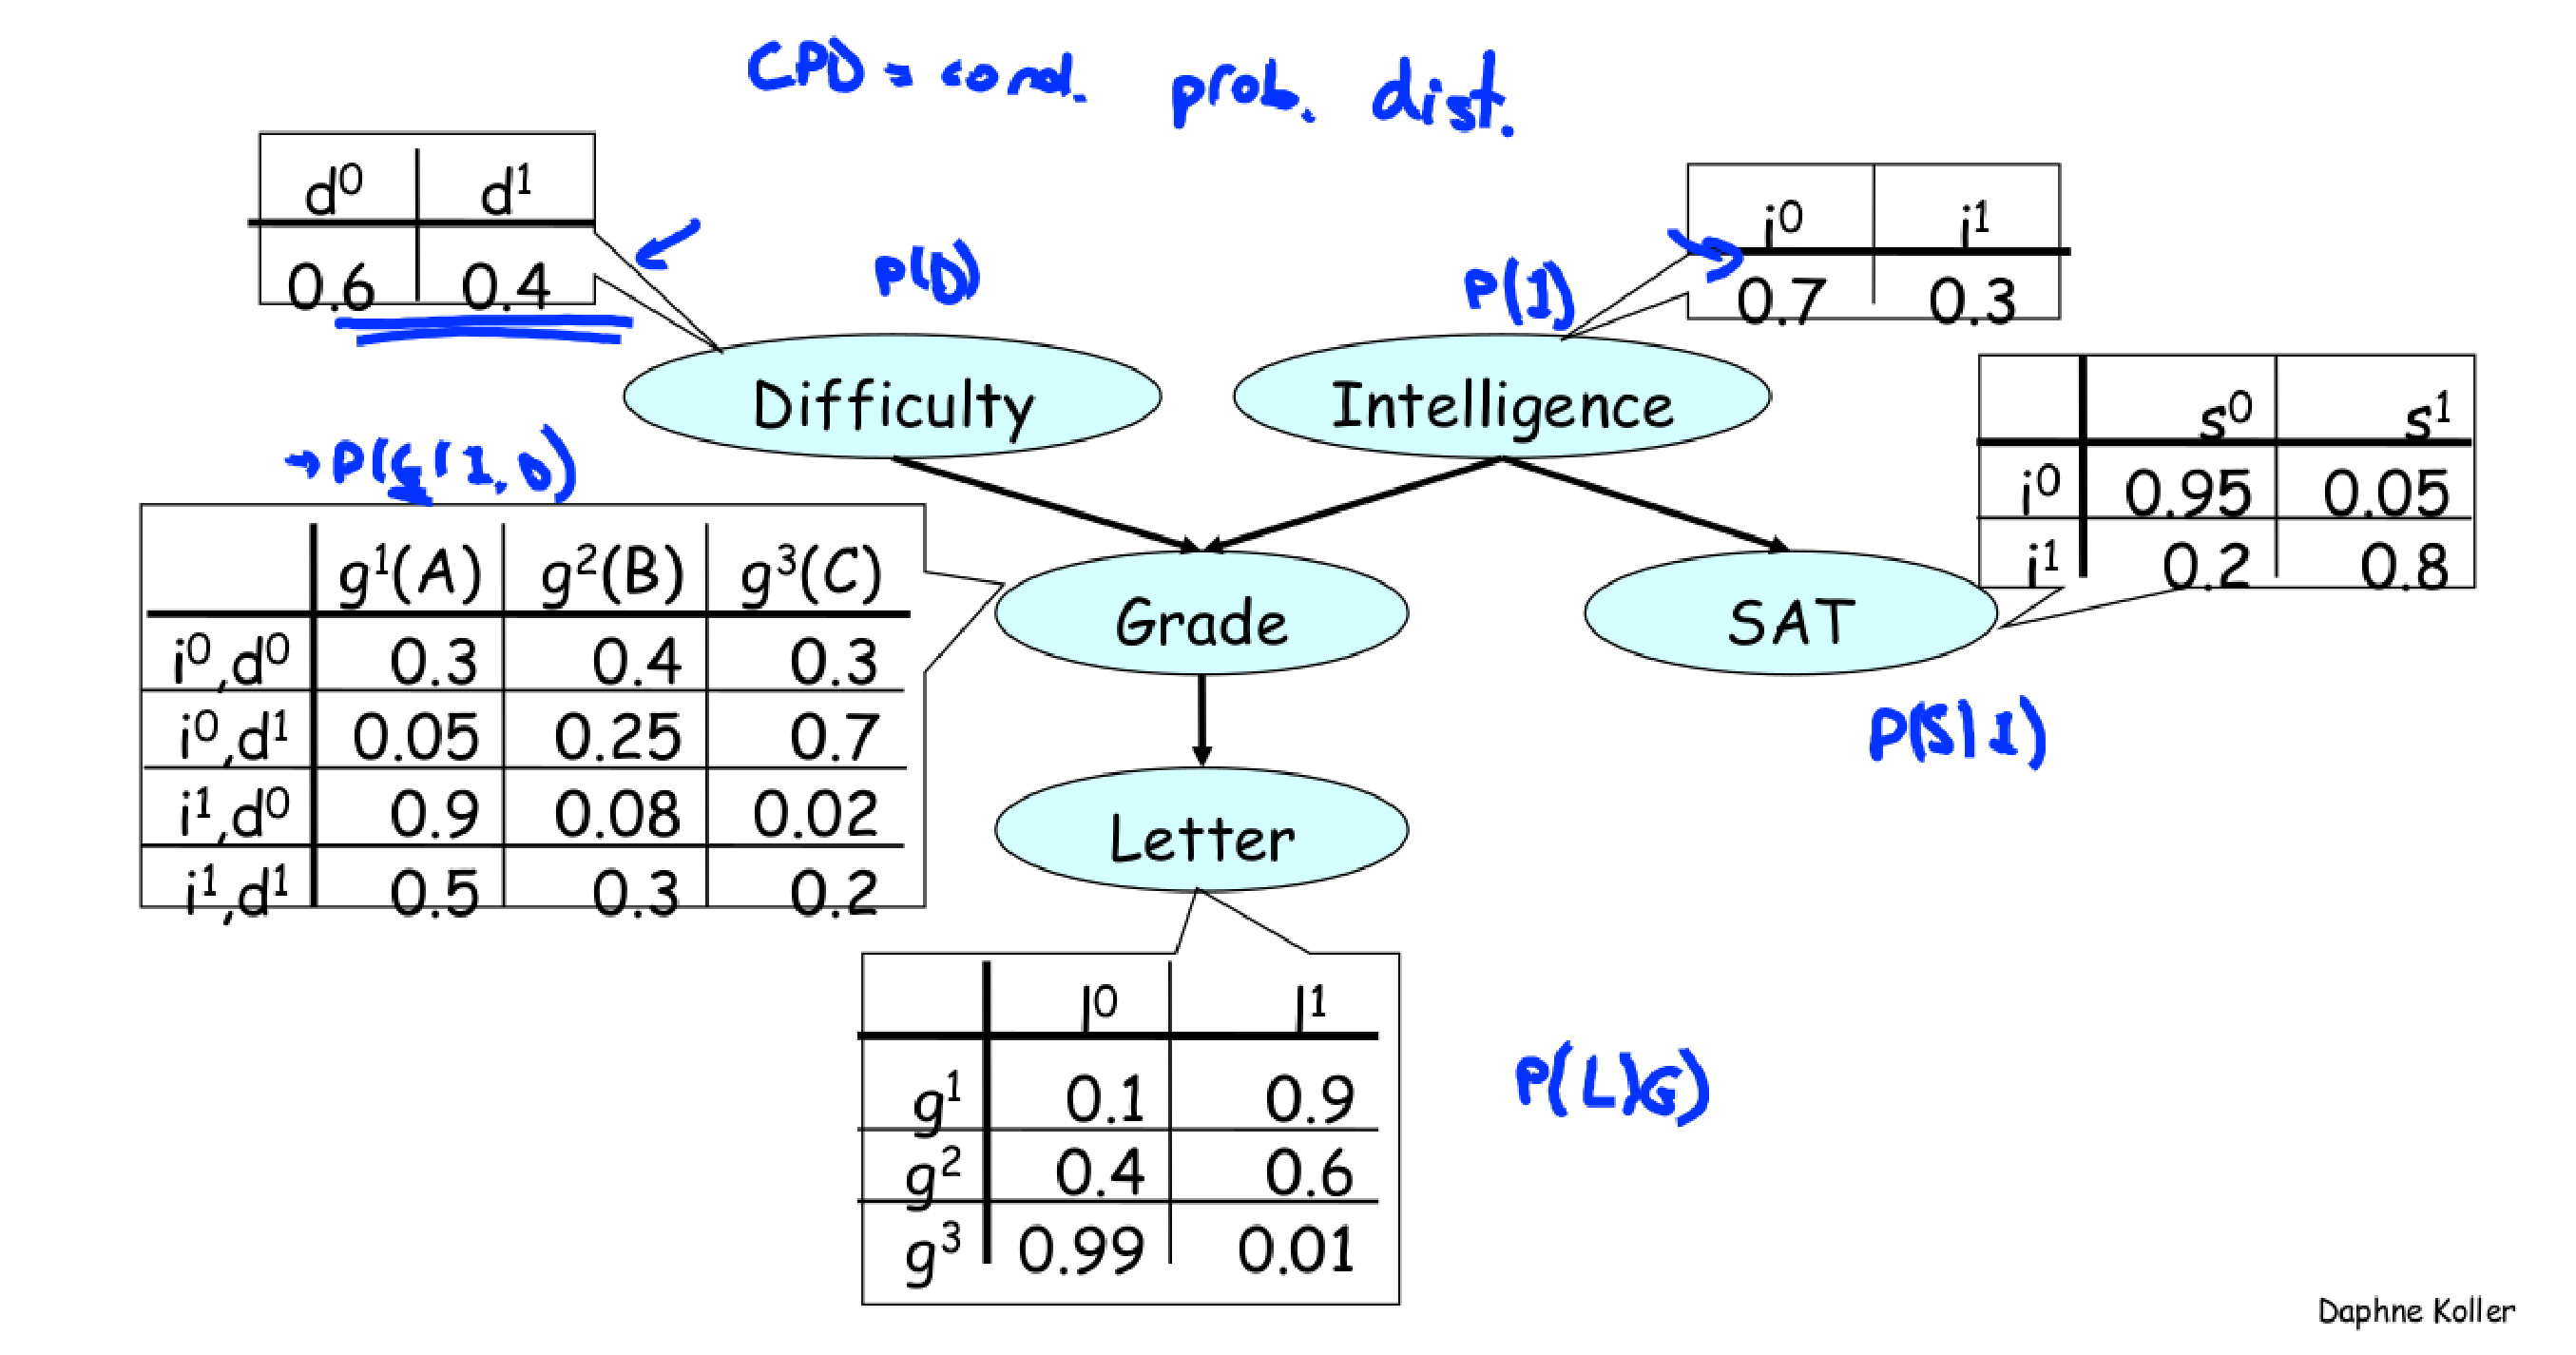
\includegraphics[scale = 0.3]{w1graphCPD}
\caption[Dependency Graph]{Dependency Graph: $D \rightarrow G$, $I \rightarrow G$, $I \rightarrow S$, $G \rightarrow L$}
\label{w1graphCPD}
\end{figure}


\subsection{Bayesian Network Definition}
Bayesian Network is:
\begin{itemize}
	\item a directed acyclic graph (DAG) G whose nodes represent the random variables $X_1,..,X_n$
	\item for each node $X_i$, there is a CPD: $P(X_i | Parents_G(X_i))$
	\item represents a joint distribution via the chain rule for Bayesian Networks in formula \ref{formChainRule} 
	\begin{align}\label{formChainRule}
	P(X_1,..,X_n) = \prod_i P(X_i|Parents_G(X_i))
	\end{align}
	\myaligns{Bayesian Network Definition}
\end{itemize}
We can prove that Bayesian Network is a legal distribution meaning it satisfies $P \geq 0$ and $\sum_i P(X_i) = 1$. The first one is trivial. The second one is proved as follow:
\begin{align*}
\sum_{D,I,G,S,L} P(D,I,G,S,L) 	&= \sum_{D,I,G,S,L} P(D)P(I)P(G|I,D)P(S|I)P(L|G) \\
								&= \sum_{D,I,G,S} P(D)P(I)P(G|I,D)P(S|I) \sum_L P(L|G) \\
								&= \sum_{D,I,G,S} P(D)P(I)P(G|I,D)P(S|I) * 1\\
								&= \sum_{D,I,G} P(D)P(I)P(G|I,D) \sum_S P(S|I)\\
								&= \sum_{D,I} P(D)P(I) \sum_G P(G|I,D)\\
								&= ...\\
								&= 1
\end{align*}

Another notation: Let G be a graph over $X_1, .., X_n$. A distribution $P$ is called to factorize over graph G if:
\begin{align*}
P(X_1, .., X_n) = \prod_i P(X_i | Par_G(X_i))
\end{align*}

\section{Reasoning Patterns}

\subsection{Causal Reasoning}
In a Bayesian network, if there is a path from one random variable to another, then the variable at the root of the path is said to affect the other random variables in the path via causal reasoning. For example, if $A \rightarrow B \rightarrow C$, then $A$ affects $B$ and $C$ via causal reasoning and $P(C)$ is generally \textbf{not equal} to $P(C|A)$.
Intuitively, inference goes in causal direction (direction of edges): \textbf{top down}.

\subsection{Evidential Reasoning}
In a Bayesian network, if there is a path from one random variable to another, then the variable at the end of the path is said to affect the other random variables in the path via evidential reasoning. For example, if $A \rightarrow B \rightarrow C$, then $C$ affects $A$ and $B$ via evidential reasoning and $P(A)$ is generally not equal to $P(A|C)$.
Bottom up: Condition the result, ask what the probability of the initial variables was (back from the cause), using Bayes' rule.

\subsection{Inter-causal Reasoning}
Flow of information between (for example) two causes of a single effect. When you condition the result, the causes are \textbf{no longer independent}. This also works across several edges and nodes. Don't really understand "explain away"! 


\chapter{Week 2}
This is the week 1 of the course Probabilistic Graphical Models (pgm) by Prof. Daphne Koller hosted on Coursera. The week 1 covers quite a lot of notions from distribution to Bayesian Network.

\section{Distribution}
A probability distribution function (aka PDF, probability density function, probability function, or density) is a function that indicates the probability that a given random variable will take on a particular value. If a random variable is discrete (i.e. the value of the random variable is contained in a countable set of values), then the probability density function, $f(x)$ of a random variable $X$ is: $f(x) = P(X = x)$.

The multivariate form of a probability distribution function is the probability that a list of random variables will take on a list of values. If the random variables are discrete, the \textbf{joint probability density function}, $f(x_1, x_2, …, x_n)$ for random variables $X_1, X_2, ..., X_n$ is defined by: 
\begin{align}
f(x_1, x_2, \ldots, x_n) = P(X_1=x_1, X_2=x_2, \ldots, X_n=x_n)
\end{align}
\myaligns{Joint Distribution}

\section{Factors}
A factor is a function or a table or a mapping from every assignment of arguments to a real value. We define below factor $\Phi(X_1, \ldots, X_k)$ where $(X_1, \ldots, X_k)$ which is the scope (a set of random variables).
\begin{align}
\Phi: Val(X_1, \ldots, X_k) \rightarrow \mathbb{R}
\end{align}
\myaligns{Factor Definition}

\subsection{Examples of Factor}
Hence, according to the definition above, a joint distribution is a factor. Figure \ref{w1JointDistri} illustrates a joint distribution $P(I,D,G)$ where $I$, $D$, $G$ represents intelligence of a student $(0, 1)$, difficulty of a course $(0,1)$, and the final grade $(A,B,C)$ that student got from that course respectively.
\begin{figure}[!ht]
\centering
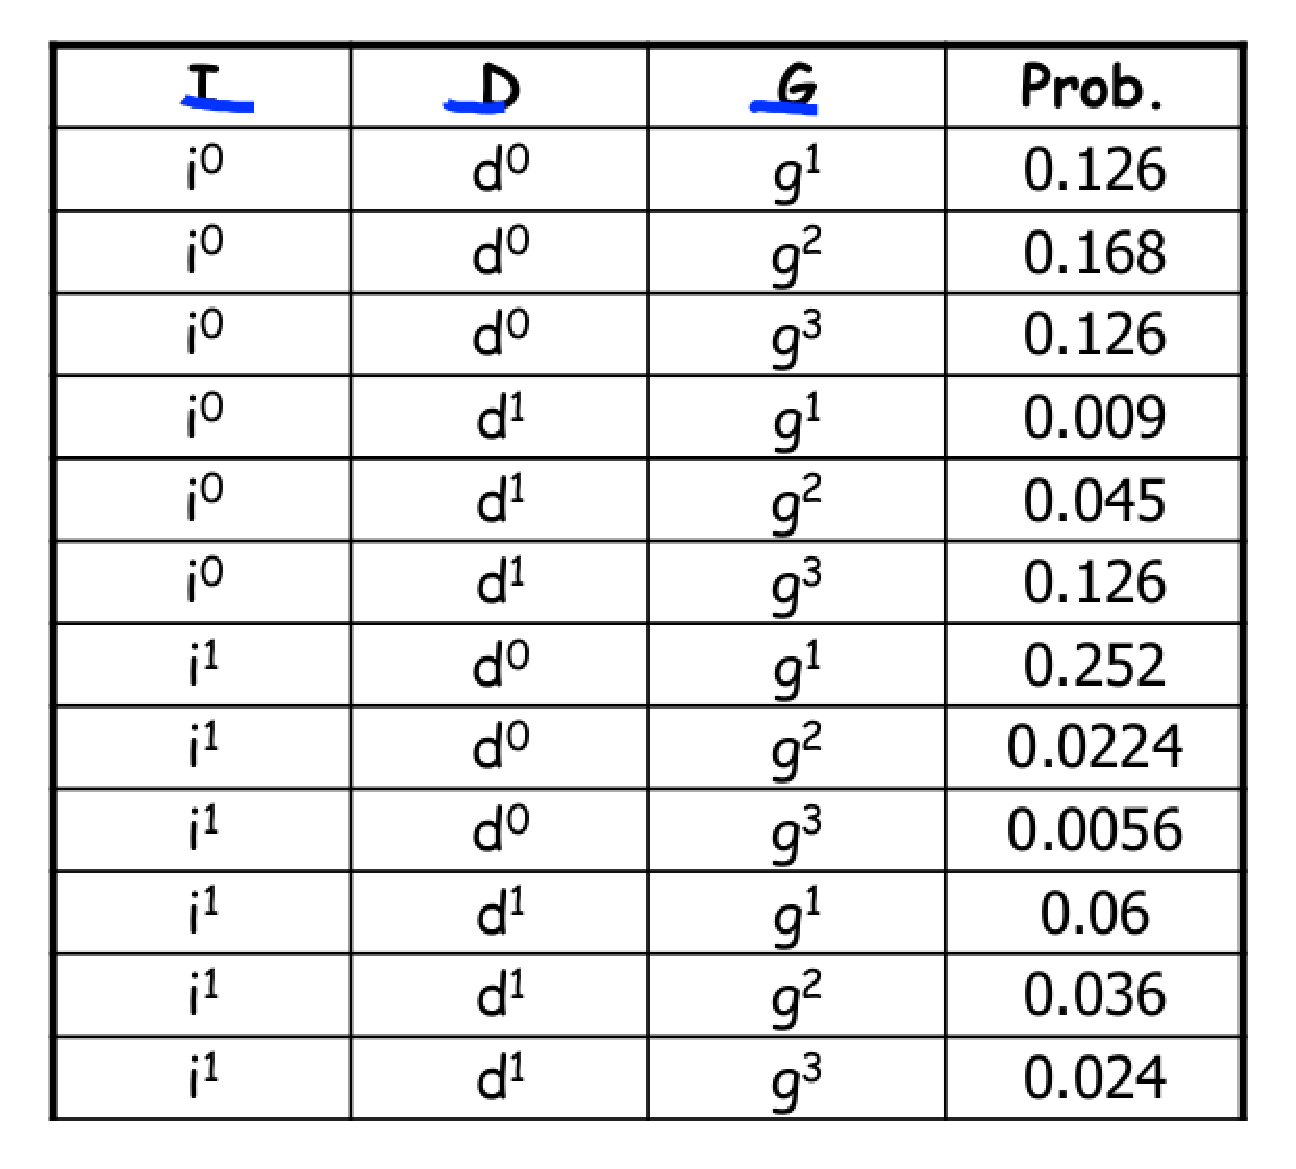
\includegraphics[scale = 0.3]{w1JointDistri}
\caption{Joint Distribution}
\label{w1JointDistri}
\end{figure}

Another example is UnnormaliCed Measure $P(I,D,g^1)$ which has scope $(I,D)$ because $G$ is always fixed to $g^1$. Another \textbf{important example} is Conditional Probability Distribution (CPD). Figure \ref{w1CPD} illustrates the \textbf{CPD} $P(G | I, D)$ which means for every combination of values to the variable $I$ and $D$, we have a probability distribution over $G$.  

\begin{figure}[!ht]
\centering
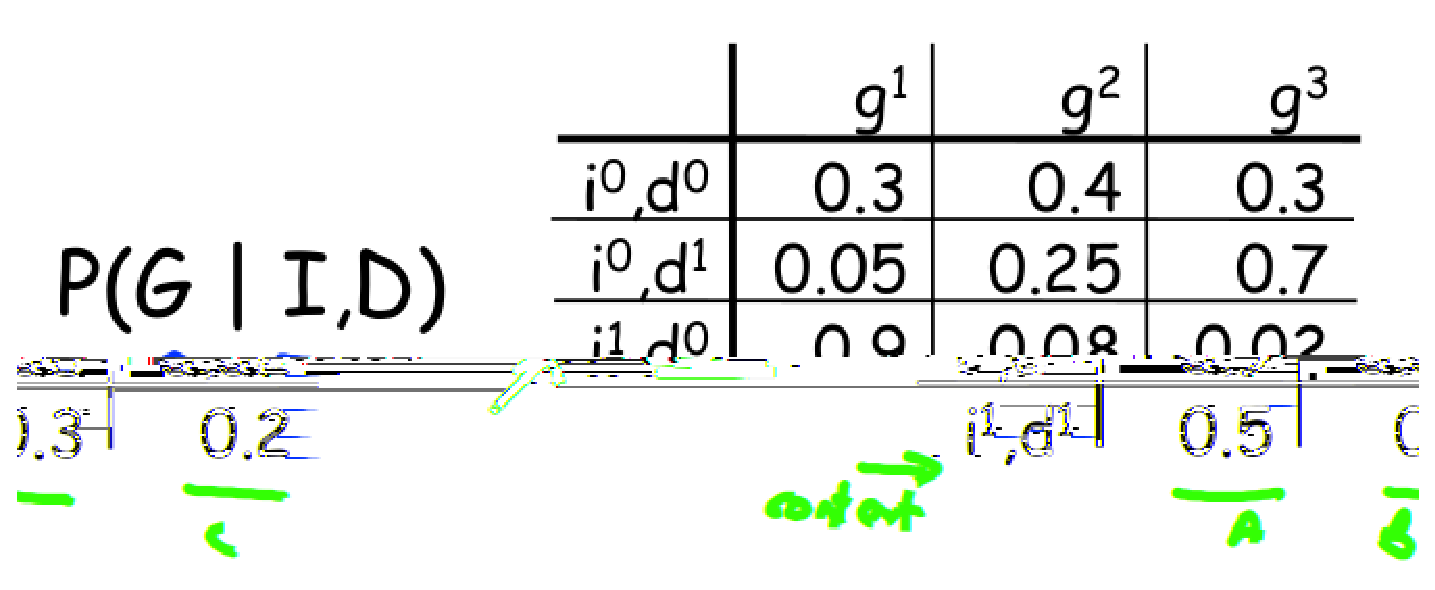
\includegraphics[scale = 0.4]{w1CPD}
\caption{Conditional Probability Distribution (CPD)}
\label{w1CPD}
\end{figure}

\section{Operations on Factors}
\subsection{Factor Products}
If $\Phi_1(A,B)$ and $\Phi_2(B,C)$ are two factors then we compute their product of $\Phi(A,B,C)$ by multiplying $\Phi_1(A,B)\Phi_2(B,C)$ for all common values of $B$ (see figure \ref{w1FactProd}).

\begin{figure}[!ht]
\centering
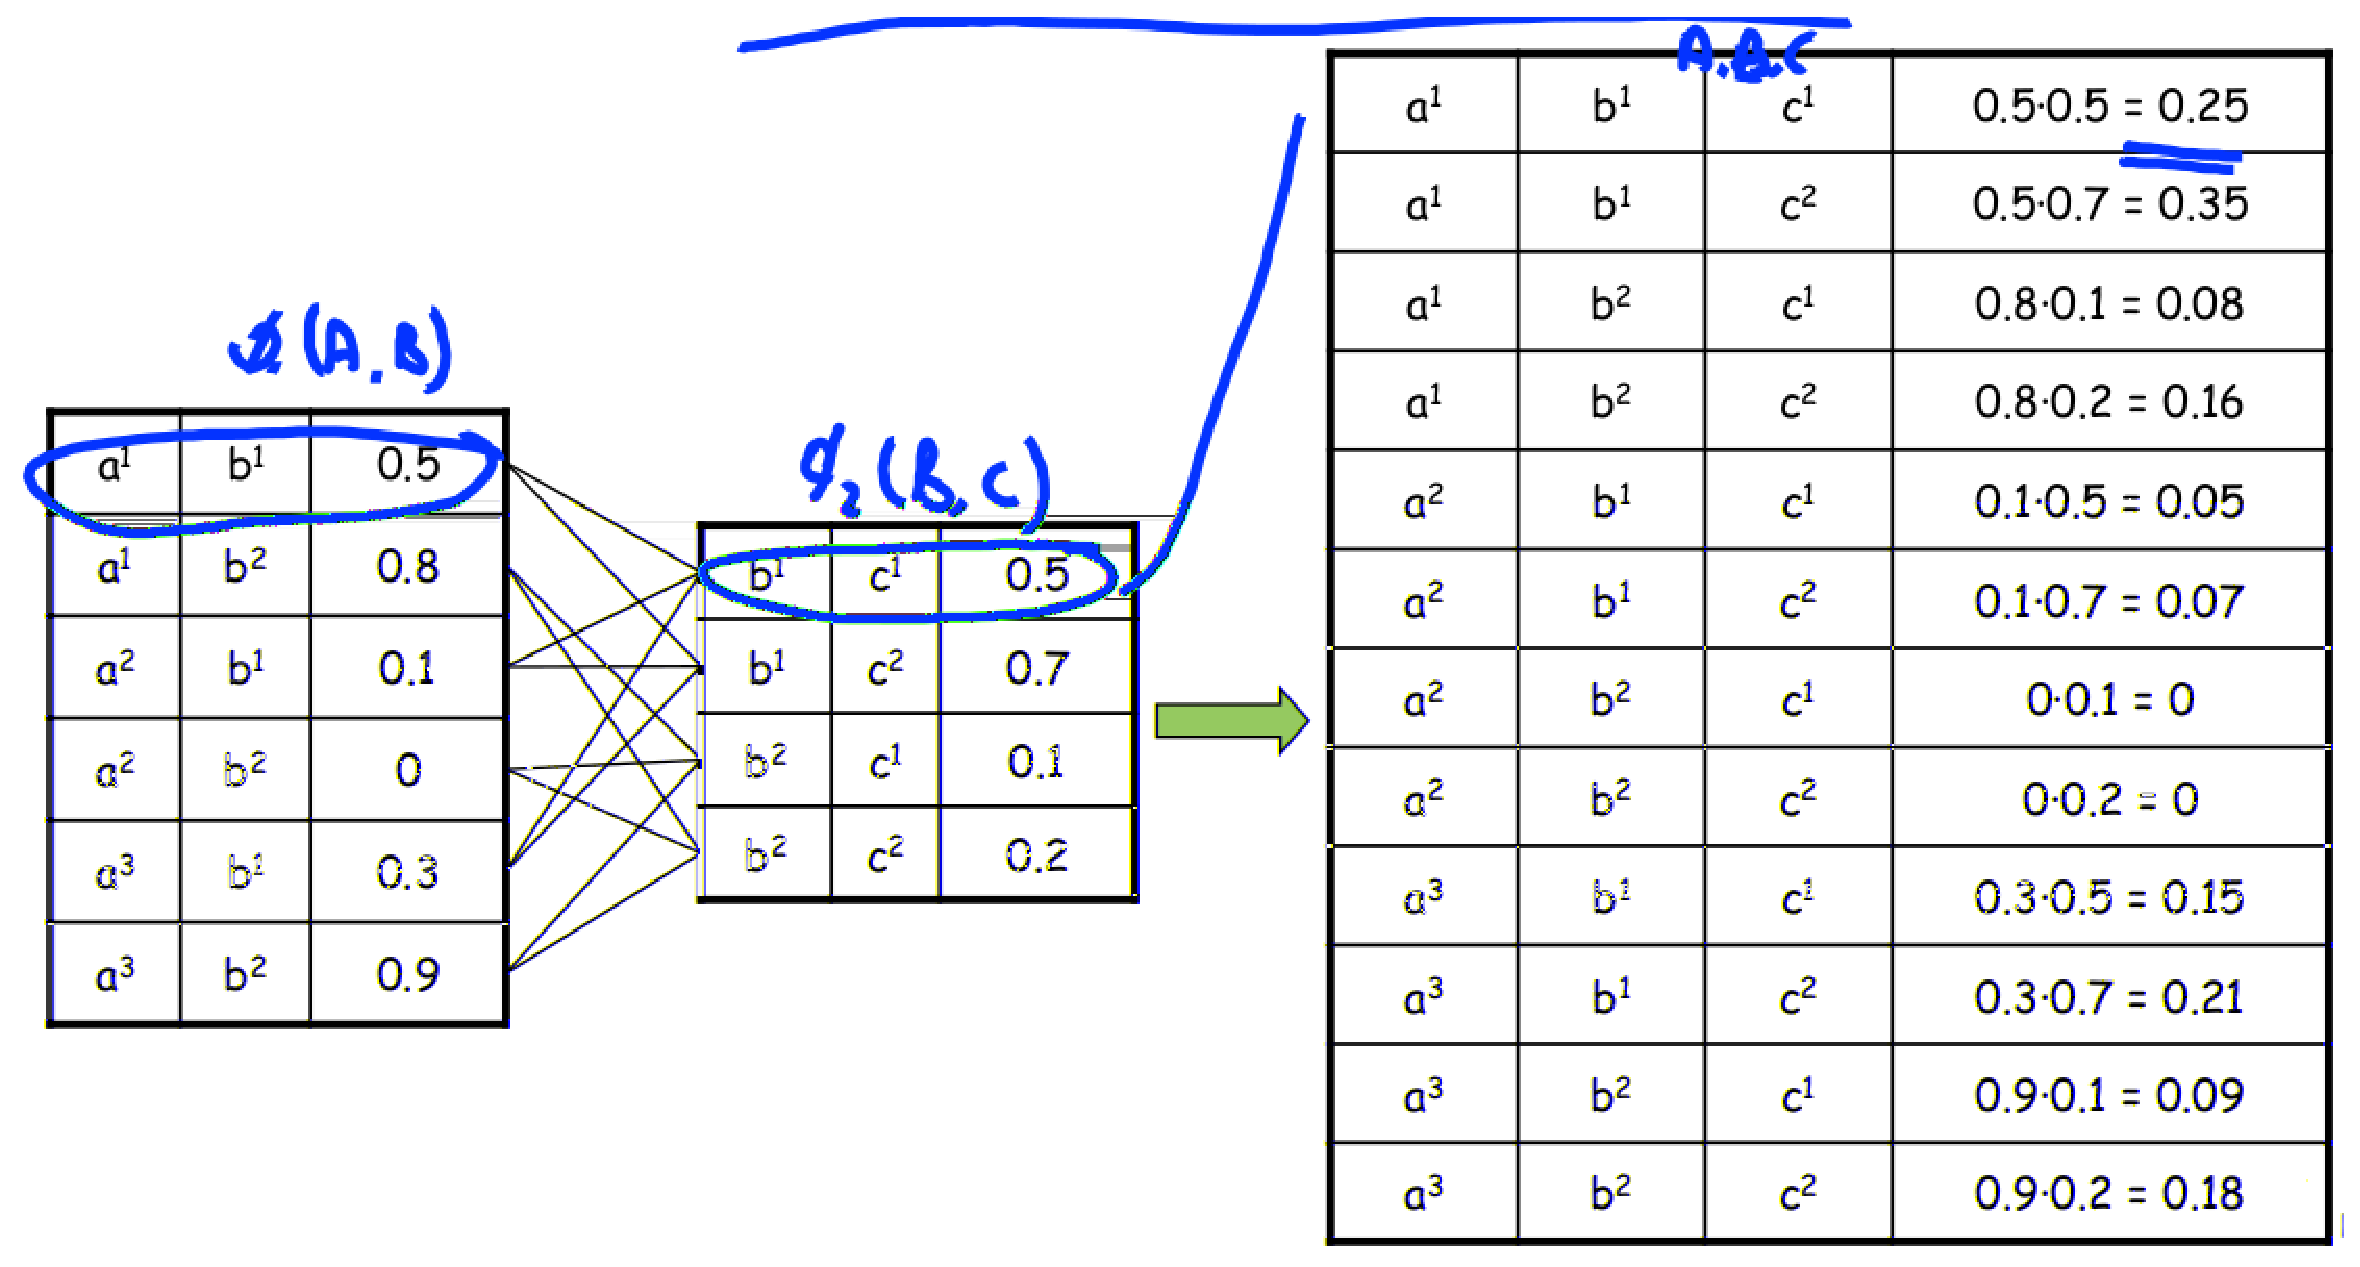
\includegraphics[scale = 0.3]{w1FactProd}
\caption{Factor Products}
\label{w1FactProd}
\end{figure}

\subsection{Factor Marginalization}
That's when we want to reduce the scope. For example, we reduce scope $(A,B,C)$ to $(A,C)$ by summing over $B$ for every assignment of $(A,C)$ (figure \ref{w1FactMarginal}).

\begin{figure}[!ht]
\centering
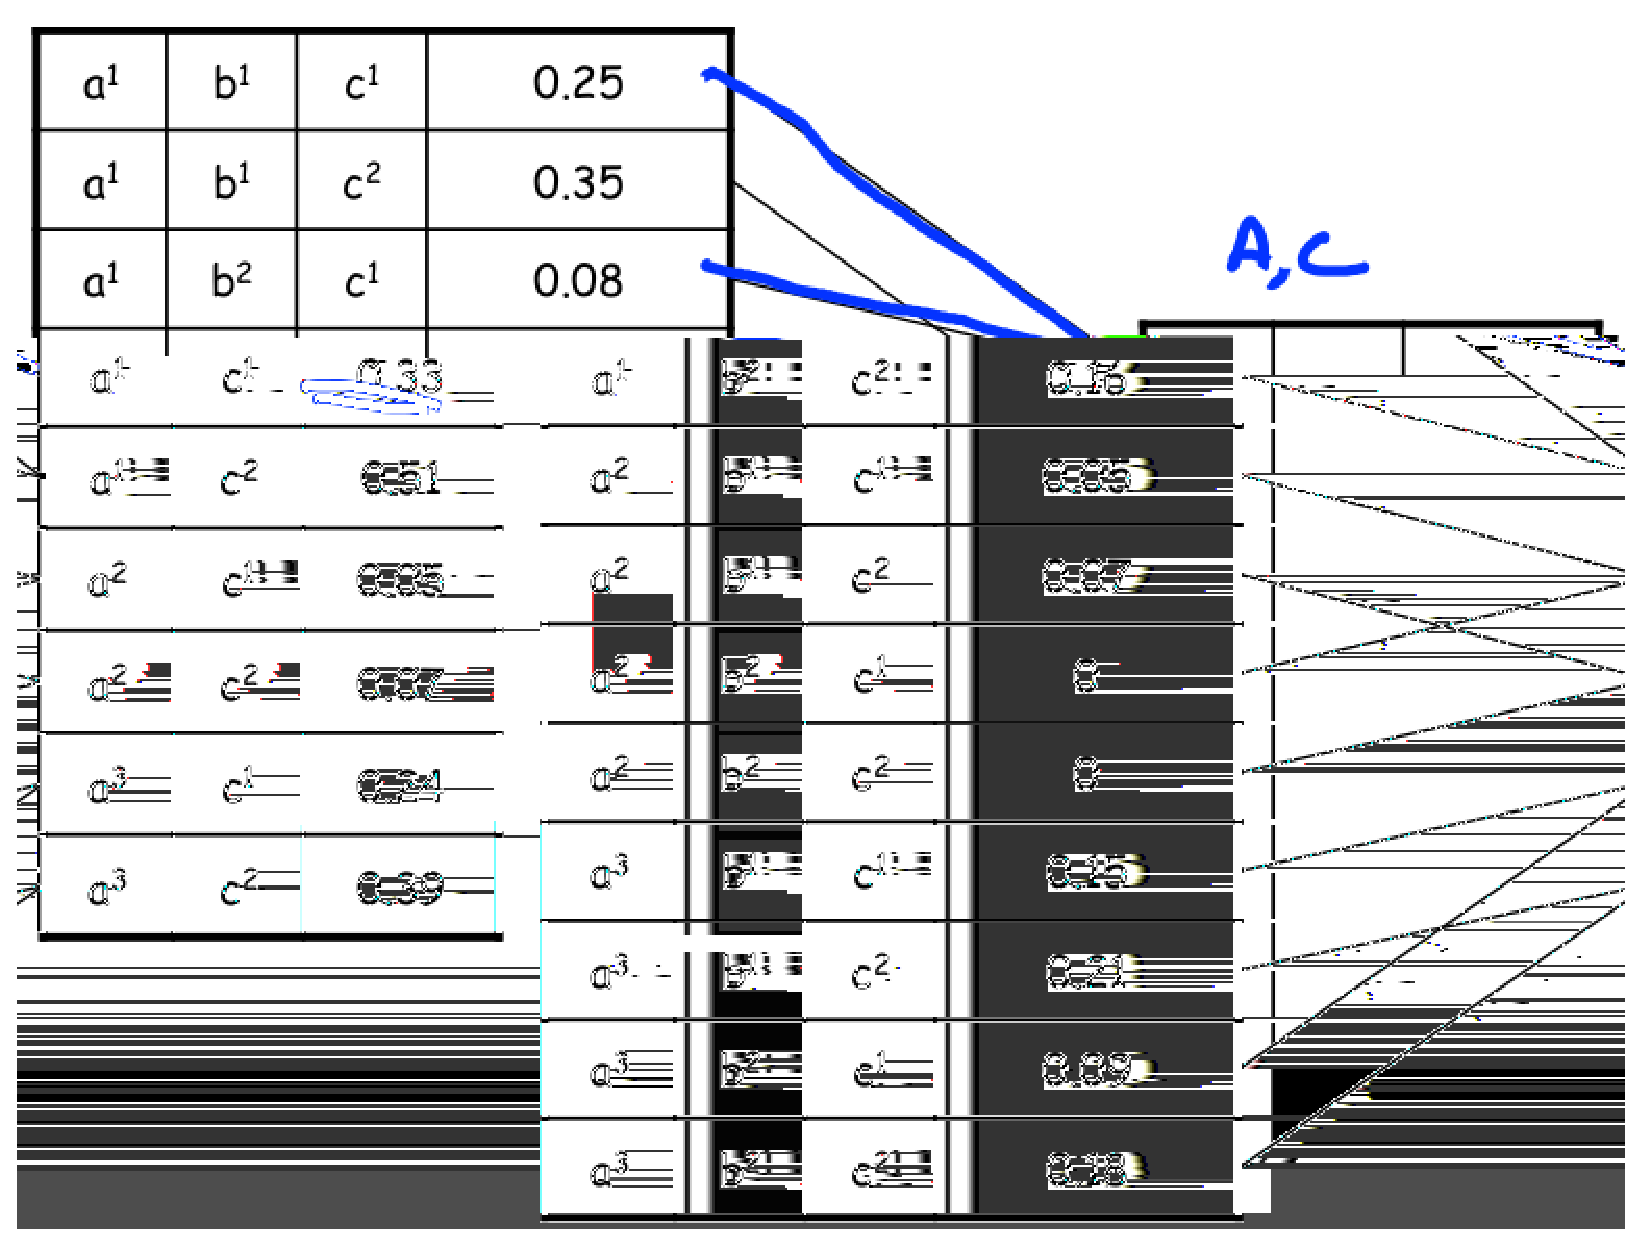
\includegraphics[scale = 0.35]{w1FactMarginal}
\caption{Factor Marginalization}
\label{w1FactMarginal}
\end{figure}

\subsection{Factor Reduction}
That's when we fix a random variable in the scope by one value (in its set of values). For example, $\Phi(A,B,C)$ is reduced to $\Phi(A,B | C = c^1)$ in illustration \ref{w1FactReduce}.
\begin{figure}[!ht]
\centering
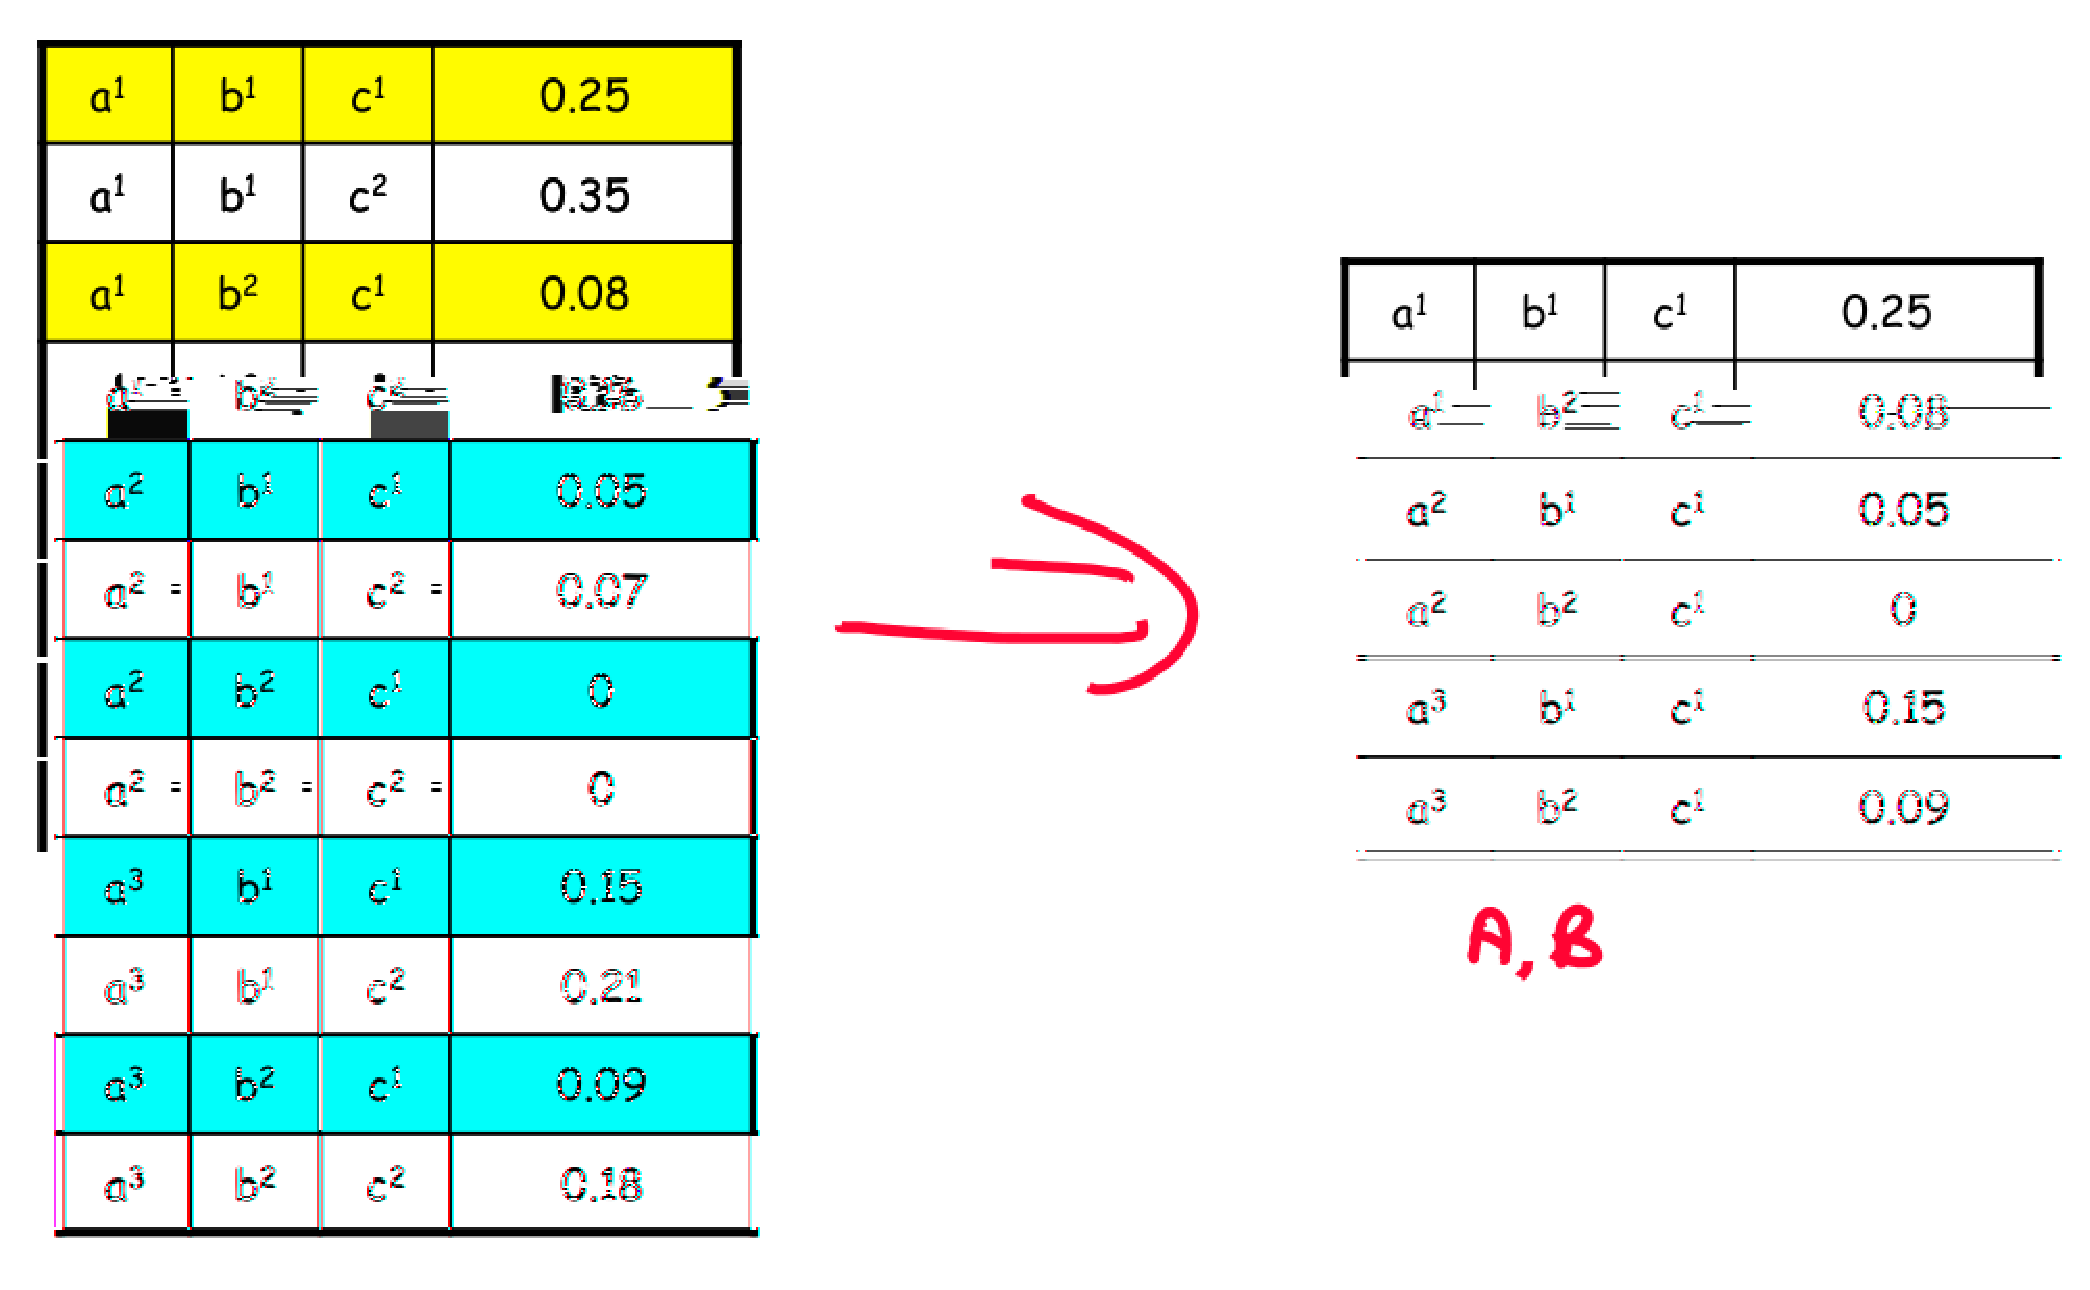
\includegraphics[scale = 0.35]{w1FactReduce}
\caption{Factor Reduction}
\label{w1FactReduce}
\end{figure}

\section{Semantics And Factorization}
\subsection{The Student Example}
The student example involving the situation where students take a course. It contains the following random variables:
\begin{itemize}
	\item Course \textbf{D}ifficulty $(D)$ ($0$ = not difficult, $1$ = difficult)
	\item Student \textbf{I}ntelligence $(I)$ ($0$ = not intelligent, $1$ = intelligent)
	\item \textbf{G}rade $(G)$ ($1$ = A, $2$ = B, $3$ = C)
	\item Student \textbf{S}AT score $(S)$ ($0$ = not good, $1$ = good)
	\item Reference \textbf{L}etter from the prof. of this course $(L)$ ($0$ = not referred, $1$ = referred)
\end{itemize}

The dependency graph is shown in figure \ref{w1graphCPD}. Intuitively, we can see the directed edge meaning a strong relation between the 2 variables. We also annotate each node of the dependency graph to a CPD (Conditional Probability Distribution). NB: I do not know where this comes from, maybe we can calculate them from the data set. We have the chain rule for Bayesian Networks in this example is described in formula below.
\begin{align}
P(G|I,D)P(S|I)P(L|G)P(D)P(I) = P(D,I,G,S,L)
\end{align}
\myaligns{Chain Rule for Bayesian Networks}

\begin{figure}[!ht]
\centering
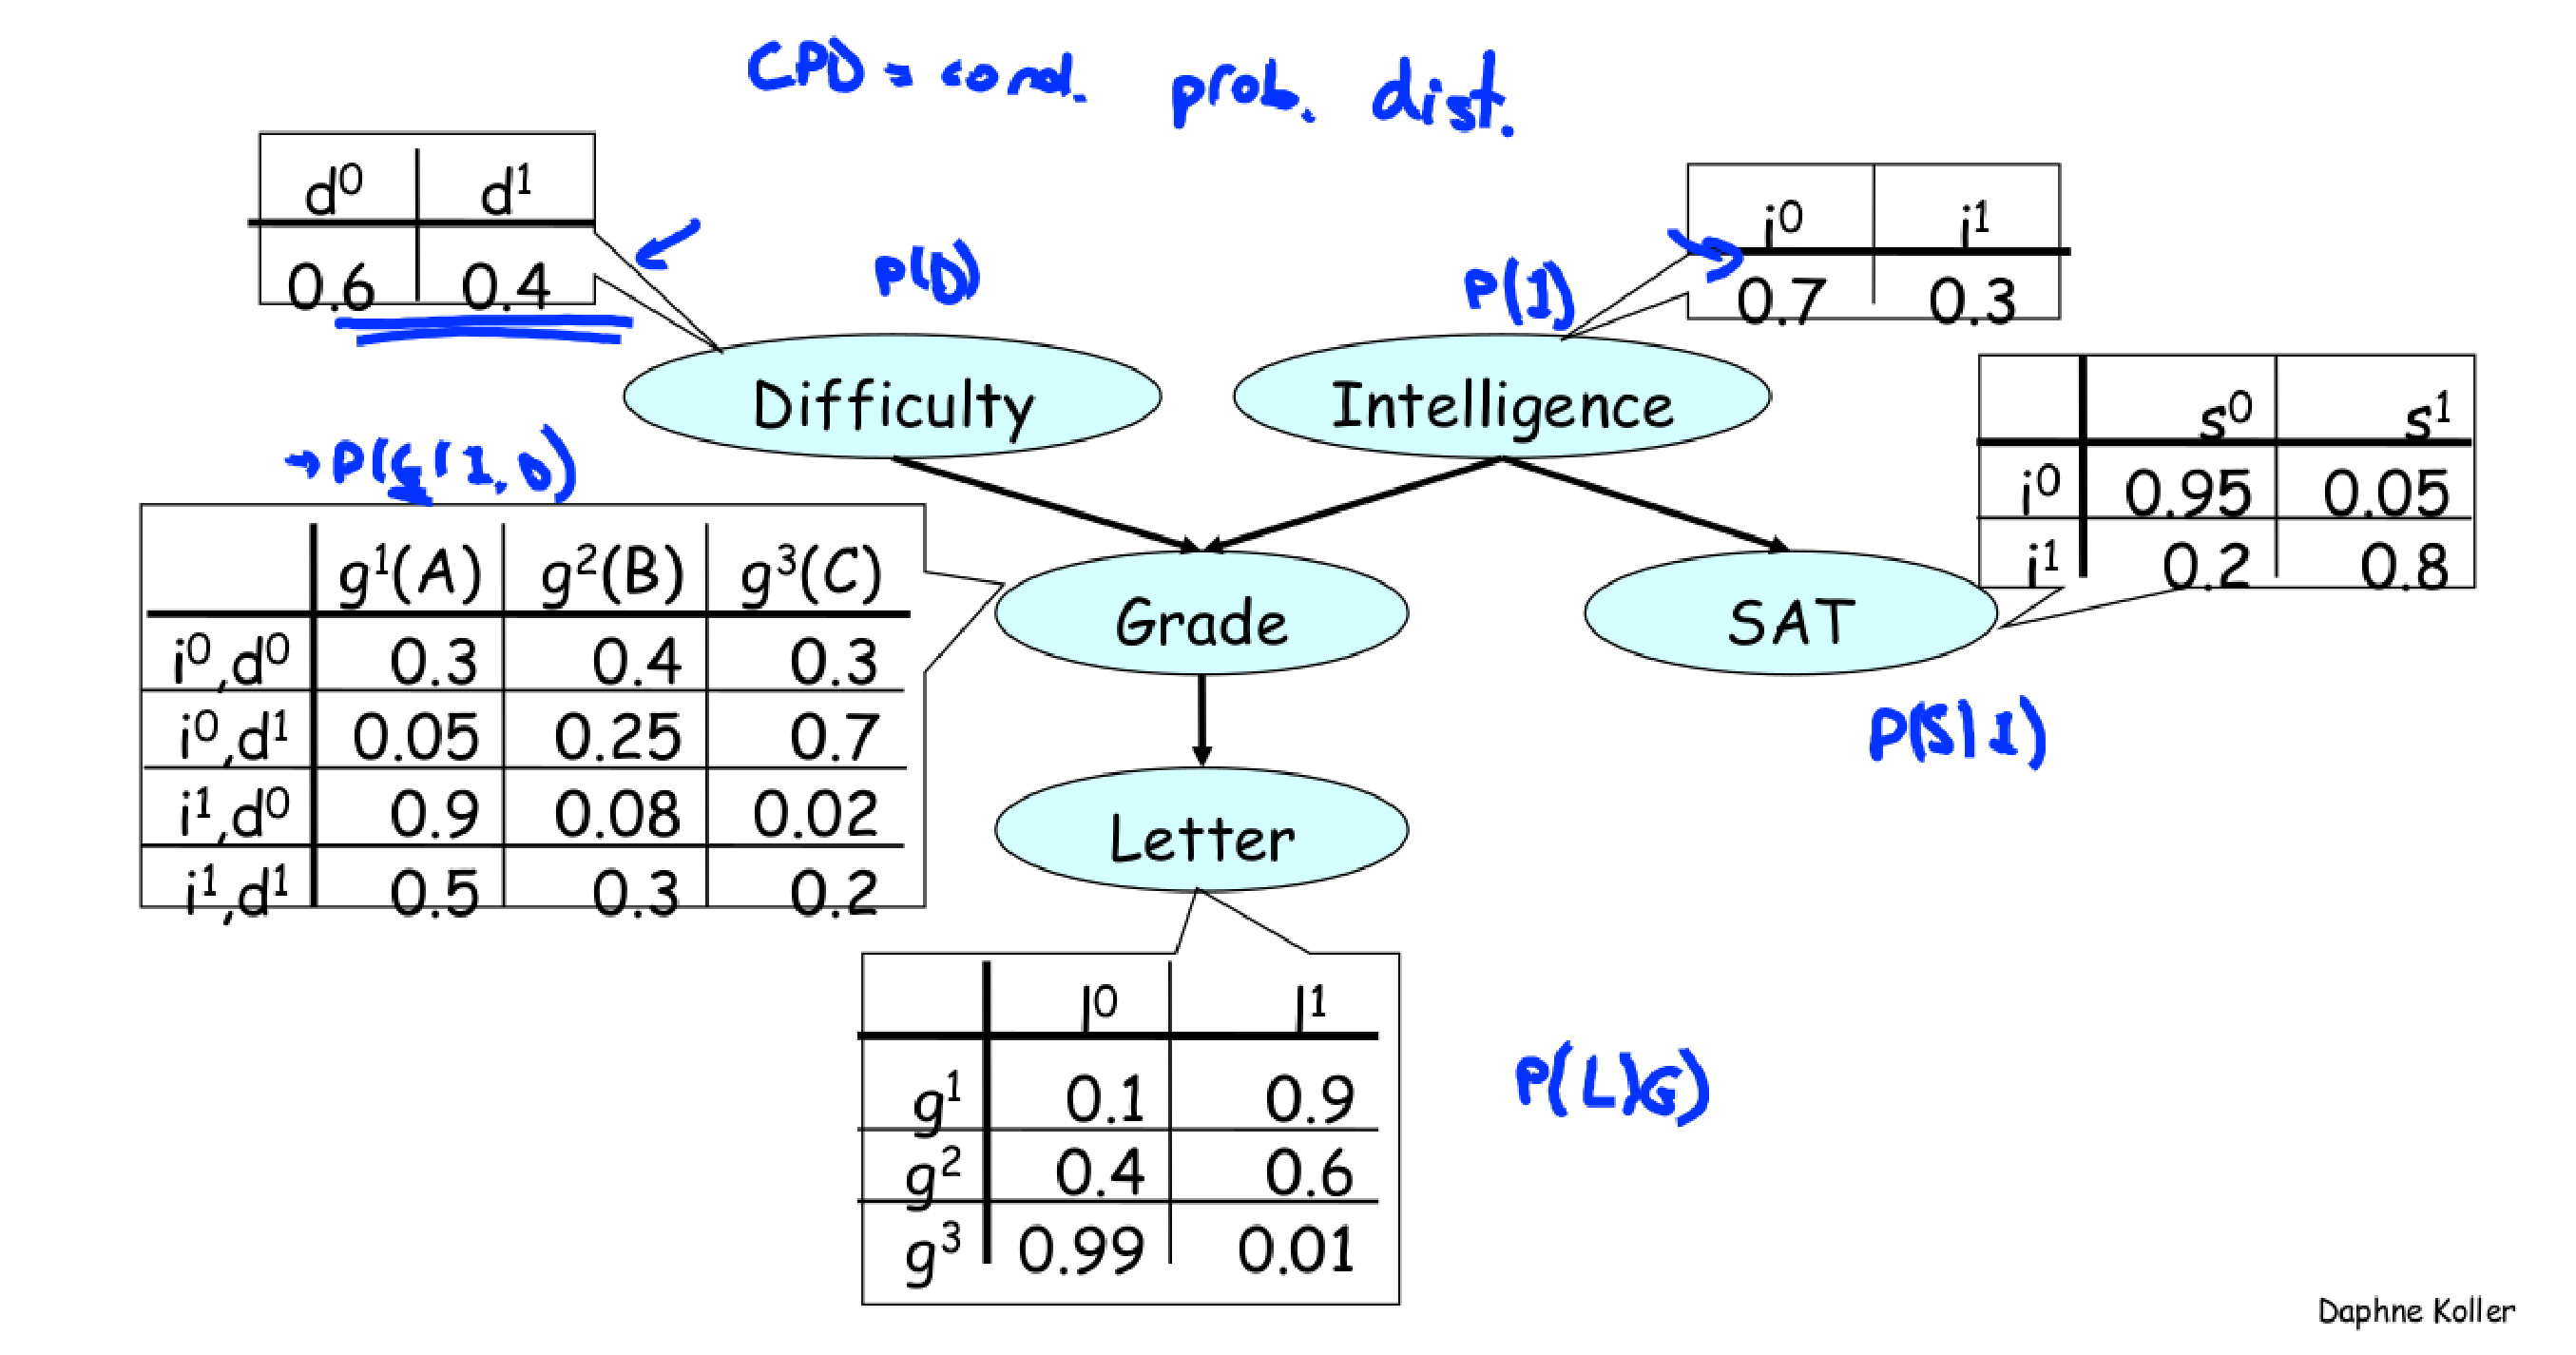
\includegraphics[scale = 0.3]{w1graphCPD}
\caption[Dependency Graph]{Dependency Graph: $D \rightarrow G$, $I \rightarrow G$, $I \rightarrow S$, $G \rightarrow L$}
\label{w1graphCPD}
\end{figure}


\subsection{Bayesian Network Definition}
Bayesian Network is:
\begin{itemize}
	\item a directed acyclic graph (DAG) G whose nodes represent the random variables $X_1,..,X_n$
	\item for each node $X_i$, there is a CPD: $P(X_i | Parents_G(X_i))$
	\item represents a joint distribution via the chain rule for Bayesian Networks in formula \ref{formChainRule} 
	\begin{align}\label{formChainRule}
	P(X_1,..,X_n) = \prod_i P(X_i|Parents_G(X_i))
	\end{align}
	\myaligns{Bayesian Network Definition}
\end{itemize}
We can prove that Bayesian Network is a legal distribution meaning it satisfies $P \geq 0$ and $\sum_i P(X_i) = 1$. The first one is trivial. The second one is proved as follow:
\begin{align*}
\sum_{D,I,G,S,L} P(D,I,G,S,L) 	&= \sum_{D,I,G,S,L} P(D)P(I)P(G|I,D)P(S|I)P(L|G) \\
								&= \sum_{D,I,G,S} P(D)P(I)P(G|I,D)P(S|I) \sum_L P(L|G) \\
								&= \sum_{D,I,G,S} P(D)P(I)P(G|I,D)P(S|I) * 1\\
								&= \sum_{D,I,G} P(D)P(I)P(G|I,D) \sum_S P(S|I)\\
								&= \sum_{D,I} P(D)P(I) \sum_G P(G|I,D)\\
								&= ...\\
								&= 1
\end{align*}

Another notation: Let G be a graph over $X_1, .., X_n$. A distribution $P$ is called to factorize over graph G if:
\begin{align*}
P(X_1, .., X_n) = \prod_i P(X_i | Par_G(X_i))
\end{align*}

\section{Reasoning Patterns}

\subsection{Causal Reasoning}
In a Bayesian network, if there is a path from one random variable to another, then the variable at the root of the path is said to affect the other random variables in the path via causal reasoning. For example, if $A \rightarrow B \rightarrow C$, then $A$ affects $B$ and $C$ via causal reasoning and $P(C)$ is generally \textbf{not equal} to $P(C|A)$.
Intuitively, inference goes in causal direction (direction of edges): \textbf{top down}.

\subsection{Evidential Reasoning}
In a Bayesian network, if there is a path from one random variable to another, then the variable at the end of the path is said to affect the other random variables in the path via evidential reasoning. For example, if $A \rightarrow B \rightarrow C$, then $C$ affects $A$ and $B$ via evidential reasoning and $P(A)$ is generally not equal to $P(A|C)$.
Bottom up: Condition the result, ask what the probability of the initial variables was (back from the cause), using Bayes' rule.

\subsection{Inter-causal Reasoning}
Flow of information between (for example) two causes of a single effect. When you condition the result, the causes are \textbf{no longer independent}. This also works across several edges and nodes. Don't really understand "explain away"! 


\chapter{Week 3}
This is the week 1 of the course Probabilistic Graphical Models (pgm) by Prof. Daphne Koller hosted on Coursera. The week 1 covers quite a lot of notions from distribution to Bayesian Network.

\section{Distribution}
A probability distribution function (aka PDF, probability density function, probability function, or density) is a function that indicates the probability that a given random variable will take on a particular value. If a random variable is discrete (i.e. the value of the random variable is contained in a countable set of values), then the probability density function, $f(x)$ of a random variable $X$ is: $f(x) = P(X = x)$.

The multivariate form of a probability distribution function is the probability that a list of random variables will take on a list of values. If the random variables are discrete, the \textbf{joint probability density function}, $f(x_1, x_2, …, x_n)$ for random variables $X_1, X_2, ..., X_n$ is defined by: 
\begin{align}
f(x_1, x_2, \ldots, x_n) = P(X_1=x_1, X_2=x_2, \ldots, X_n=x_n)
\end{align}
\myaligns{Joint Distribution}

\section{Factors}
A factor is a function or a table or a mapping from every assignment of arguments to a real value. We define below factor $\Phi(X_1, \ldots, X_k)$ where $(X_1, \ldots, X_k)$ which is the scope (a set of random variables).
\begin{align}
\Phi: Val(X_1, \ldots, X_k) \rightarrow \mathbb{R}
\end{align}
\myaligns{Factor Definition}

\subsection{Examples of Factor}
Hence, according to the definition above, a joint distribution is a factor. Figure \ref{w1JointDistri} illustrates a joint distribution $P(I,D,G)$ where $I$, $D$, $G$ represents intelligence of a student $(0, 1)$, difficulty of a course $(0,1)$, and the final grade $(A,B,C)$ that student got from that course respectively.
\begin{figure}[!ht]
\centering
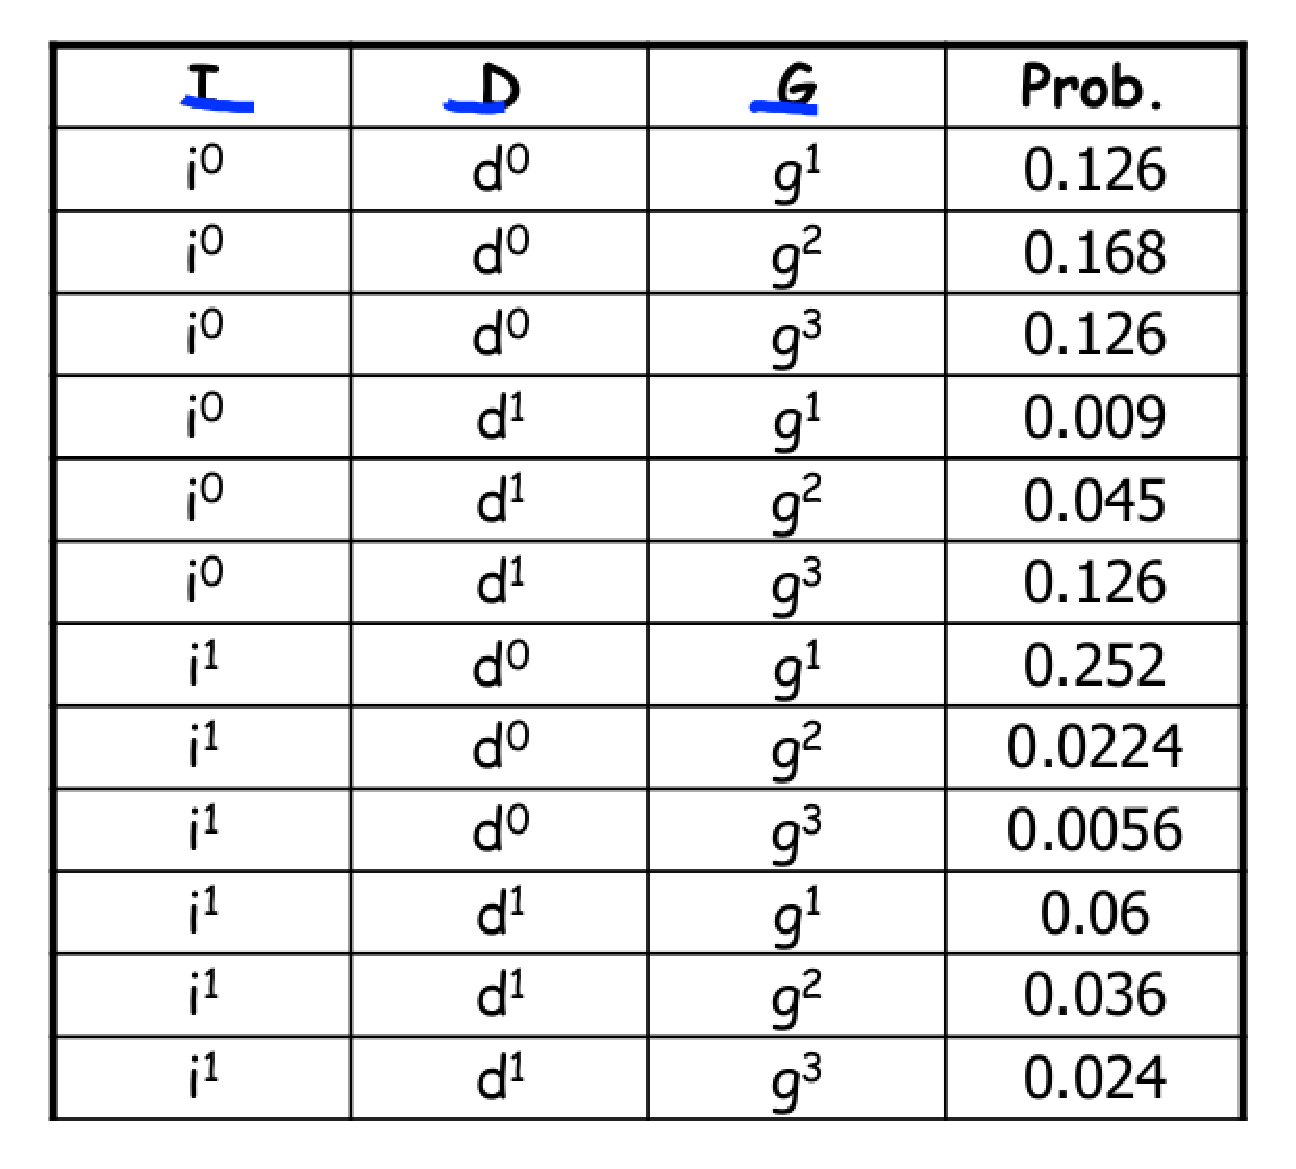
\includegraphics[scale = 0.3]{w1JointDistri}
\caption{Joint Distribution}
\label{w1JointDistri}
\end{figure}

Another example is UnnormaliCed Measure $P(I,D,g^1)$ which has scope $(I,D)$ because $G$ is always fixed to $g^1$. Another \textbf{important example} is Conditional Probability Distribution (CPD). Figure \ref{w1CPD} illustrates the \textbf{CPD} $P(G | I, D)$ which means for every combination of values to the variable $I$ and $D$, we have a probability distribution over $G$.  

\begin{figure}[!ht]
\centering
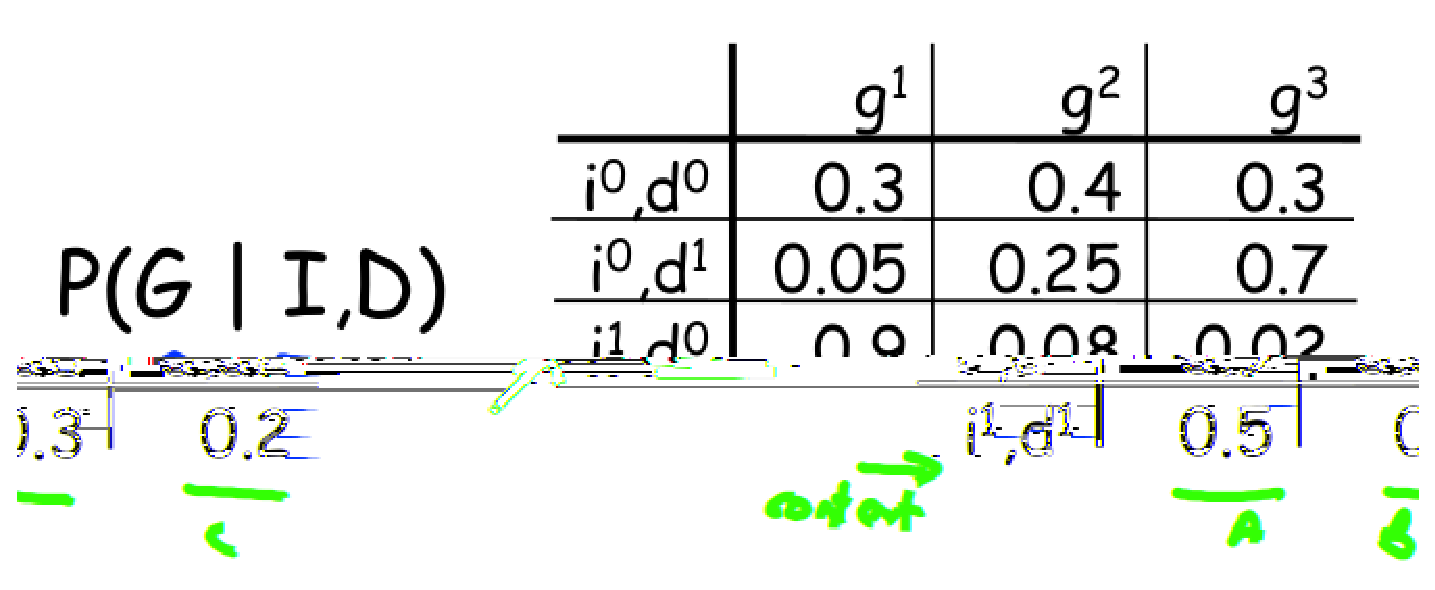
\includegraphics[scale = 0.4]{w1CPD}
\caption{Conditional Probability Distribution (CPD)}
\label{w1CPD}
\end{figure}

\section{Operations on Factors}
\subsection{Factor Products}
If $\Phi_1(A,B)$ and $\Phi_2(B,C)$ are two factors then we compute their product of $\Phi(A,B,C)$ by multiplying $\Phi_1(A,B)\Phi_2(B,C)$ for all common values of $B$ (see figure \ref{w1FactProd}).

\begin{figure}[!ht]
\centering
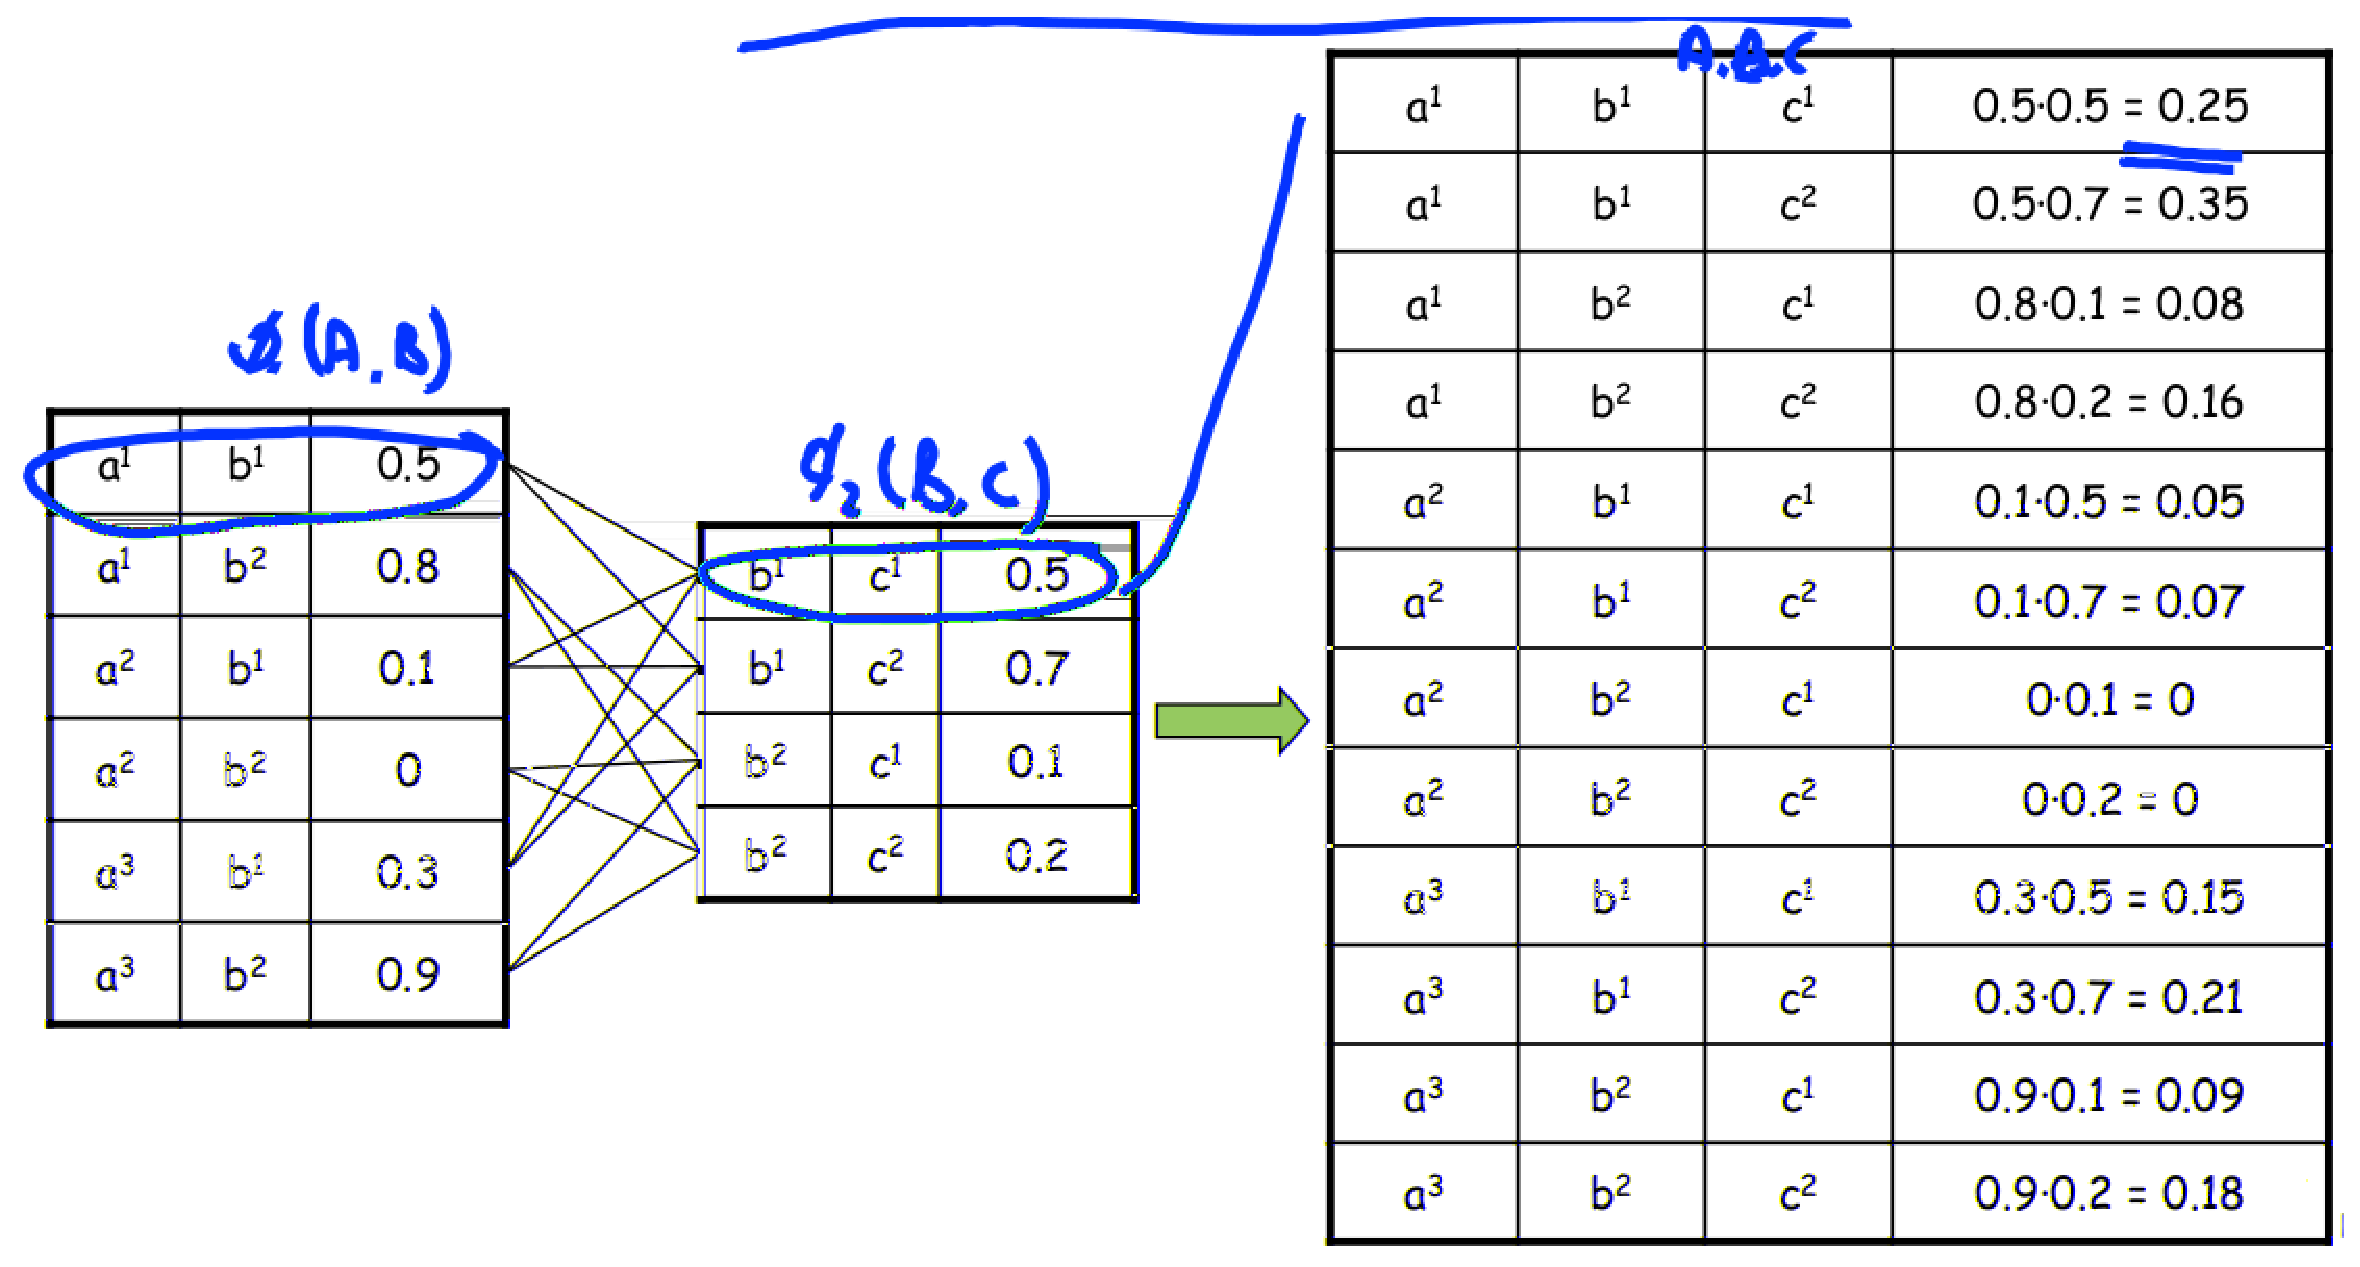
\includegraphics[scale = 0.3]{w1FactProd}
\caption{Factor Products}
\label{w1FactProd}
\end{figure}

\subsection{Factor Marginalization}
That's when we want to reduce the scope. For example, we reduce scope $(A,B,C)$ to $(A,C)$ by summing over $B$ for every assignment of $(A,C)$ (figure \ref{w1FactMarginal}).

\begin{figure}[!ht]
\centering
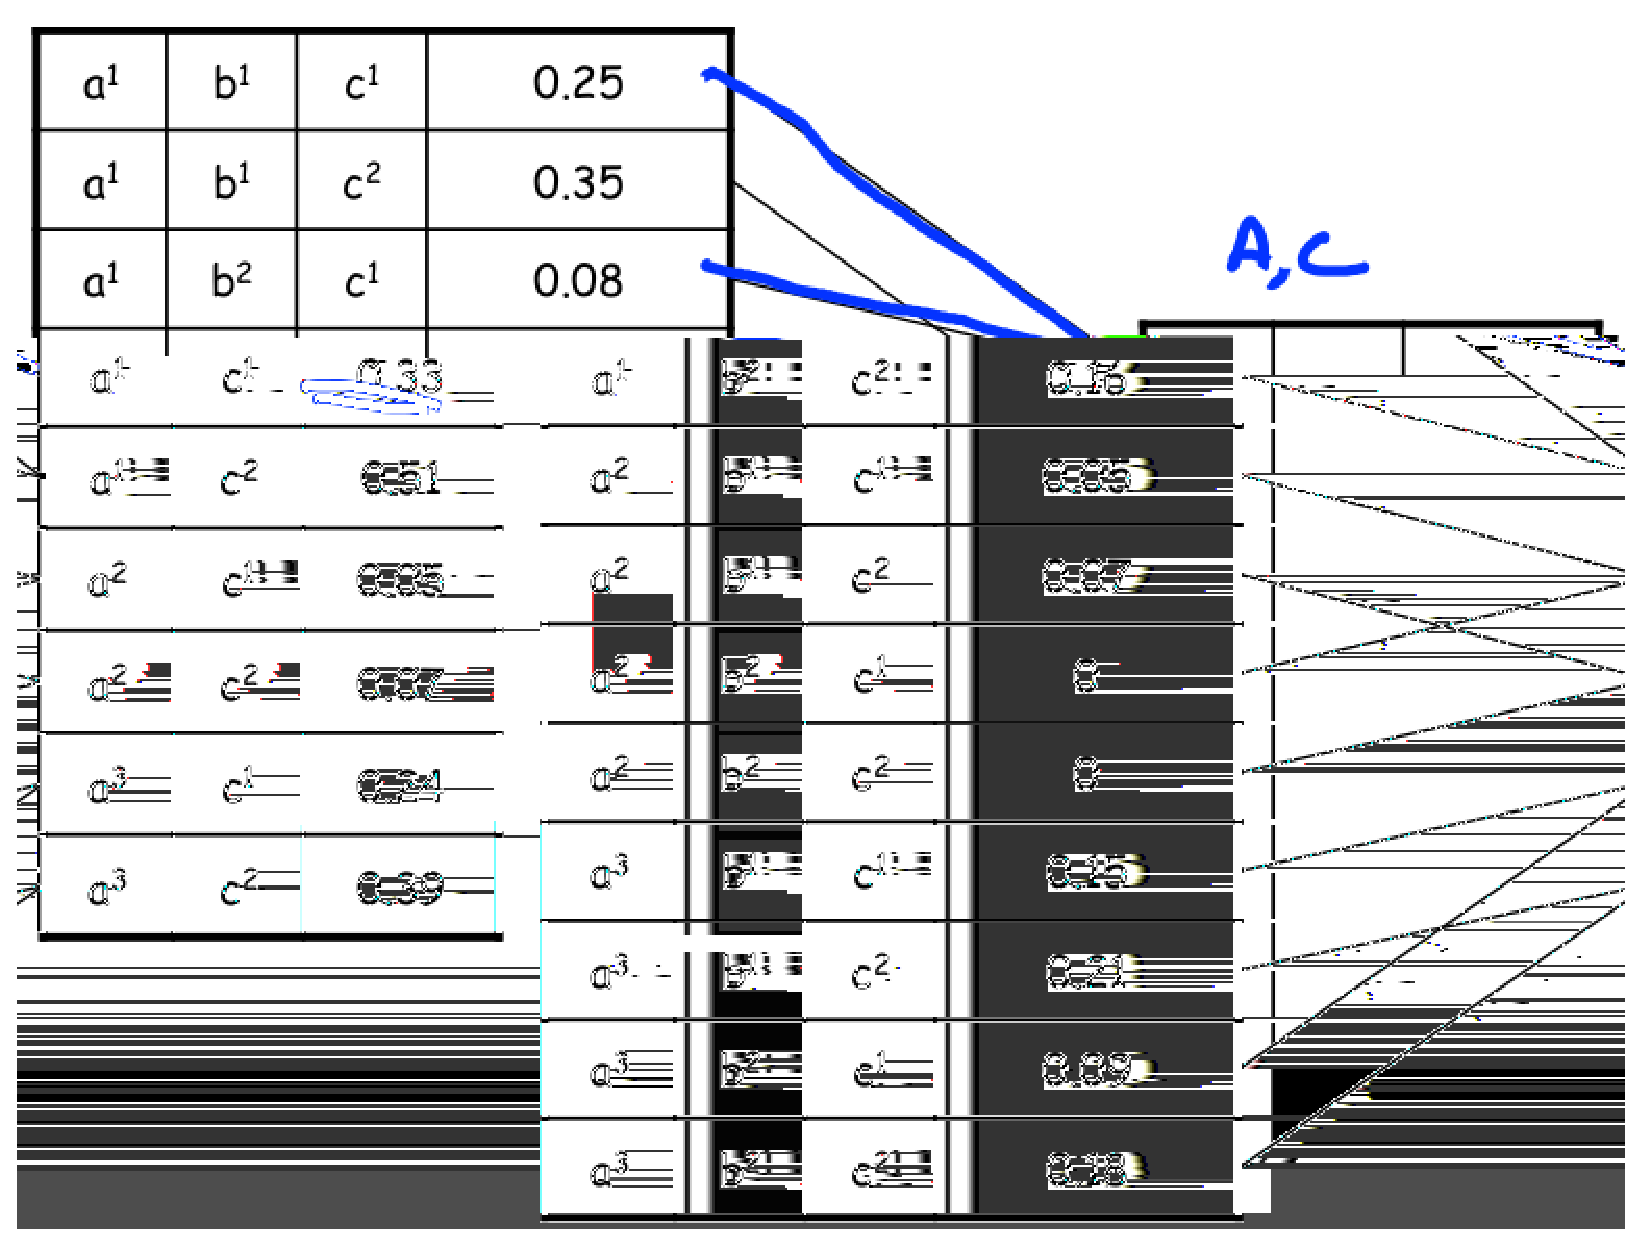
\includegraphics[scale = 0.35]{w1FactMarginal}
\caption{Factor Marginalization}
\label{w1FactMarginal}
\end{figure}

\subsection{Factor Reduction}
That's when we fix a random variable in the scope by one value (in its set of values). For example, $\Phi(A,B,C)$ is reduced to $\Phi(A,B | C = c^1)$ in illustration \ref{w1FactReduce}.
\begin{figure}[!ht]
\centering
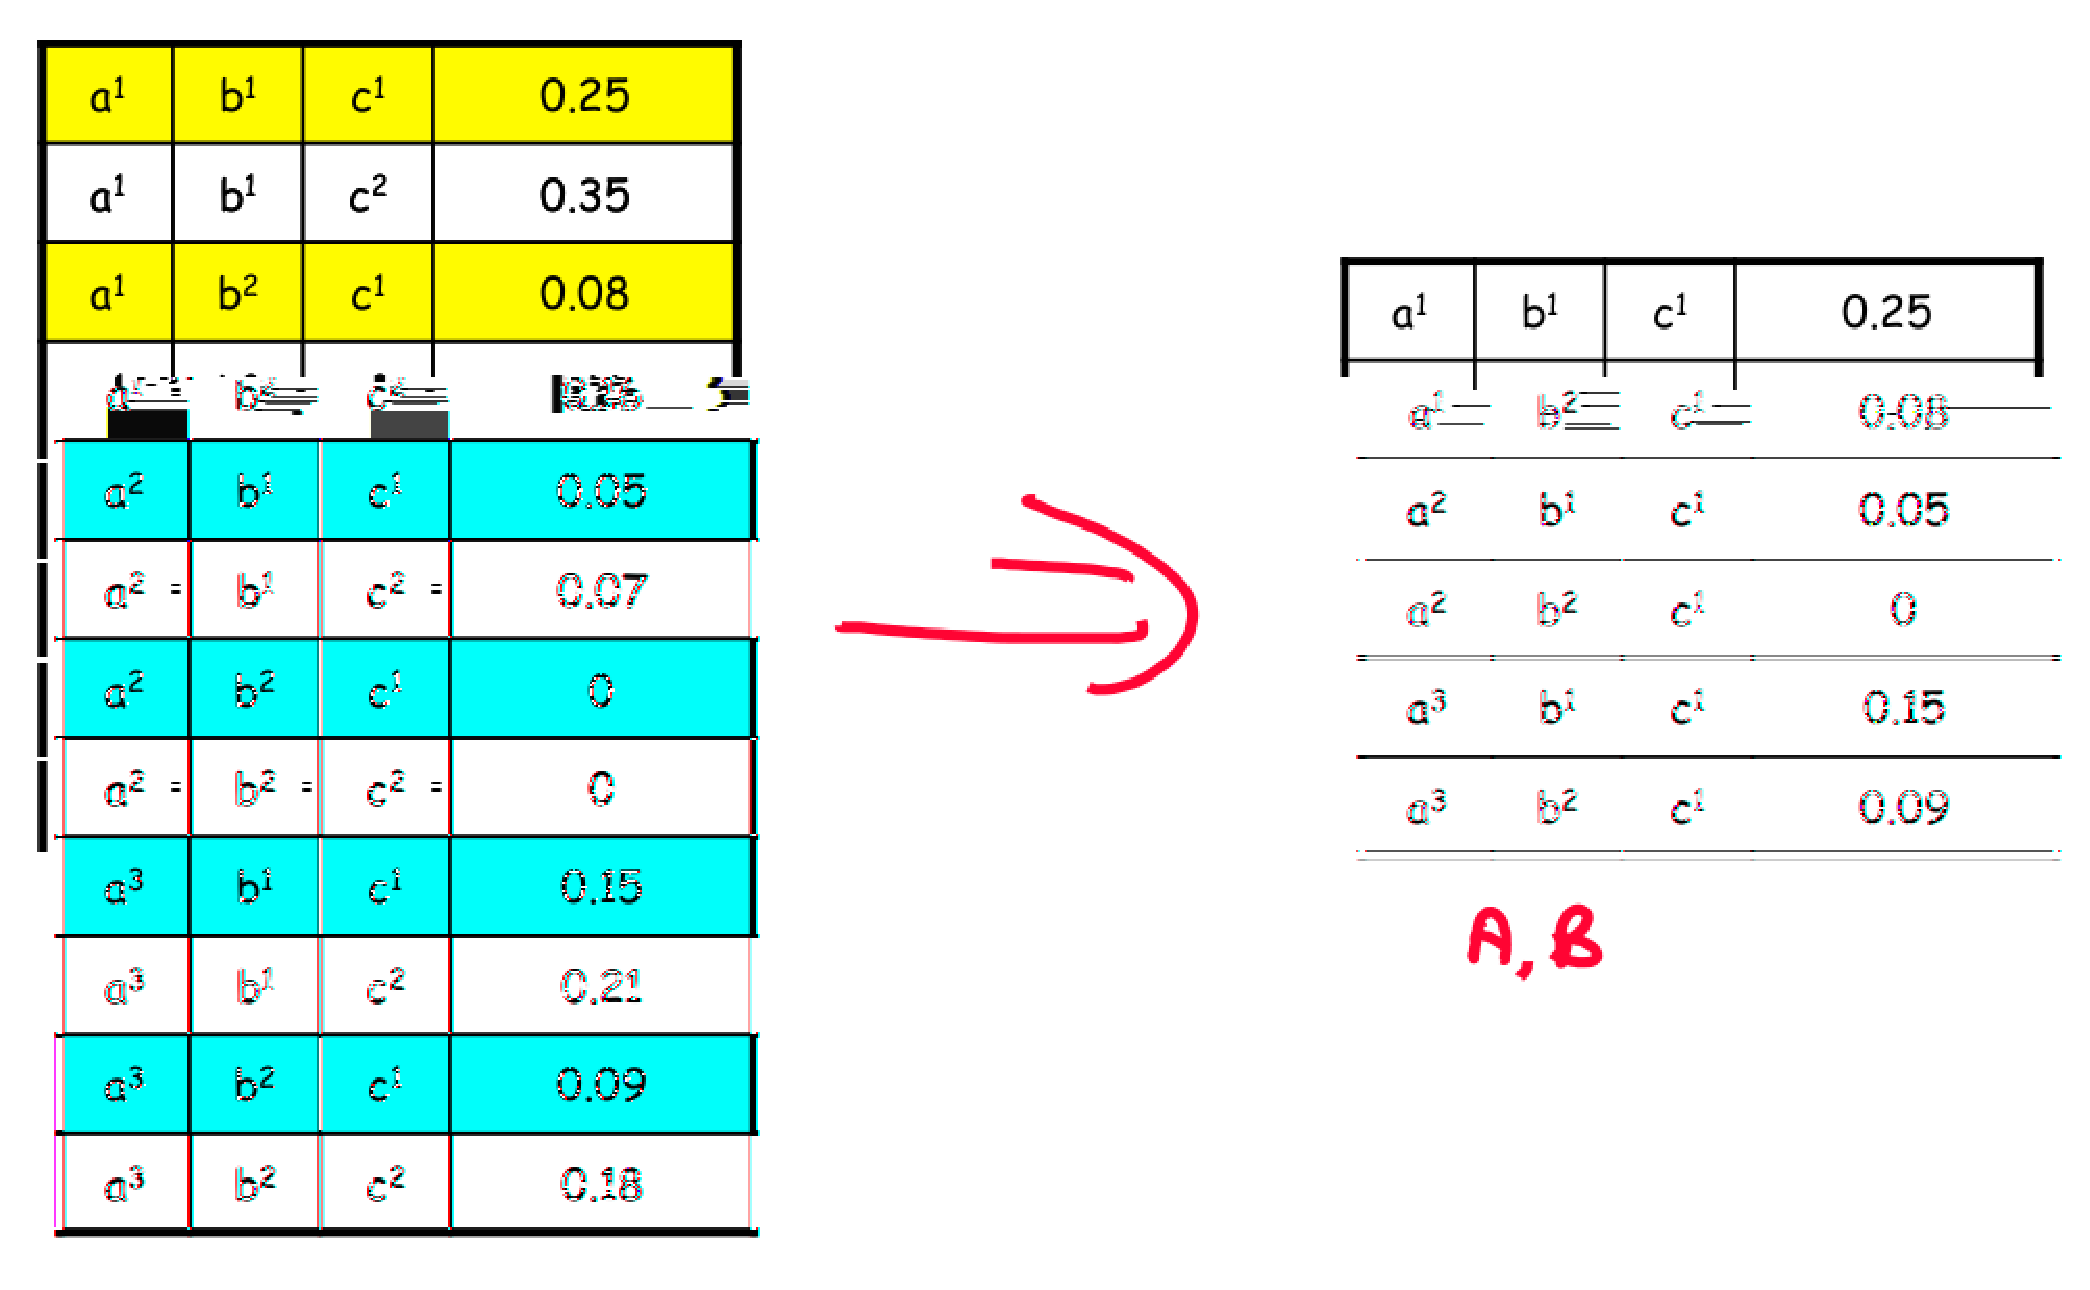
\includegraphics[scale = 0.35]{w1FactReduce}
\caption{Factor Reduction}
\label{w1FactReduce}
\end{figure}

\section{Semantics And Factorization}
\subsection{The Student Example}
The student example involving the situation where students take a course. It contains the following random variables:
\begin{itemize}
	\item Course \textbf{D}ifficulty $(D)$ ($0$ = not difficult, $1$ = difficult)
	\item Student \textbf{I}ntelligence $(I)$ ($0$ = not intelligent, $1$ = intelligent)
	\item \textbf{G}rade $(G)$ ($1$ = A, $2$ = B, $3$ = C)
	\item Student \textbf{S}AT score $(S)$ ($0$ = not good, $1$ = good)
	\item Reference \textbf{L}etter from the prof. of this course $(L)$ ($0$ = not referred, $1$ = referred)
\end{itemize}

The dependency graph is shown in figure \ref{w1graphCPD}. Intuitively, we can see the directed edge meaning a strong relation between the 2 variables. We also annotate each node of the dependency graph to a CPD (Conditional Probability Distribution). NB: I do not know where this comes from, maybe we can calculate them from the data set. We have the chain rule for Bayesian Networks in this example is described in formula below.
\begin{align}
P(G|I,D)P(S|I)P(L|G)P(D)P(I) = P(D,I,G,S,L)
\end{align}
\myaligns{Chain Rule for Bayesian Networks}

\begin{figure}[!ht]
\centering
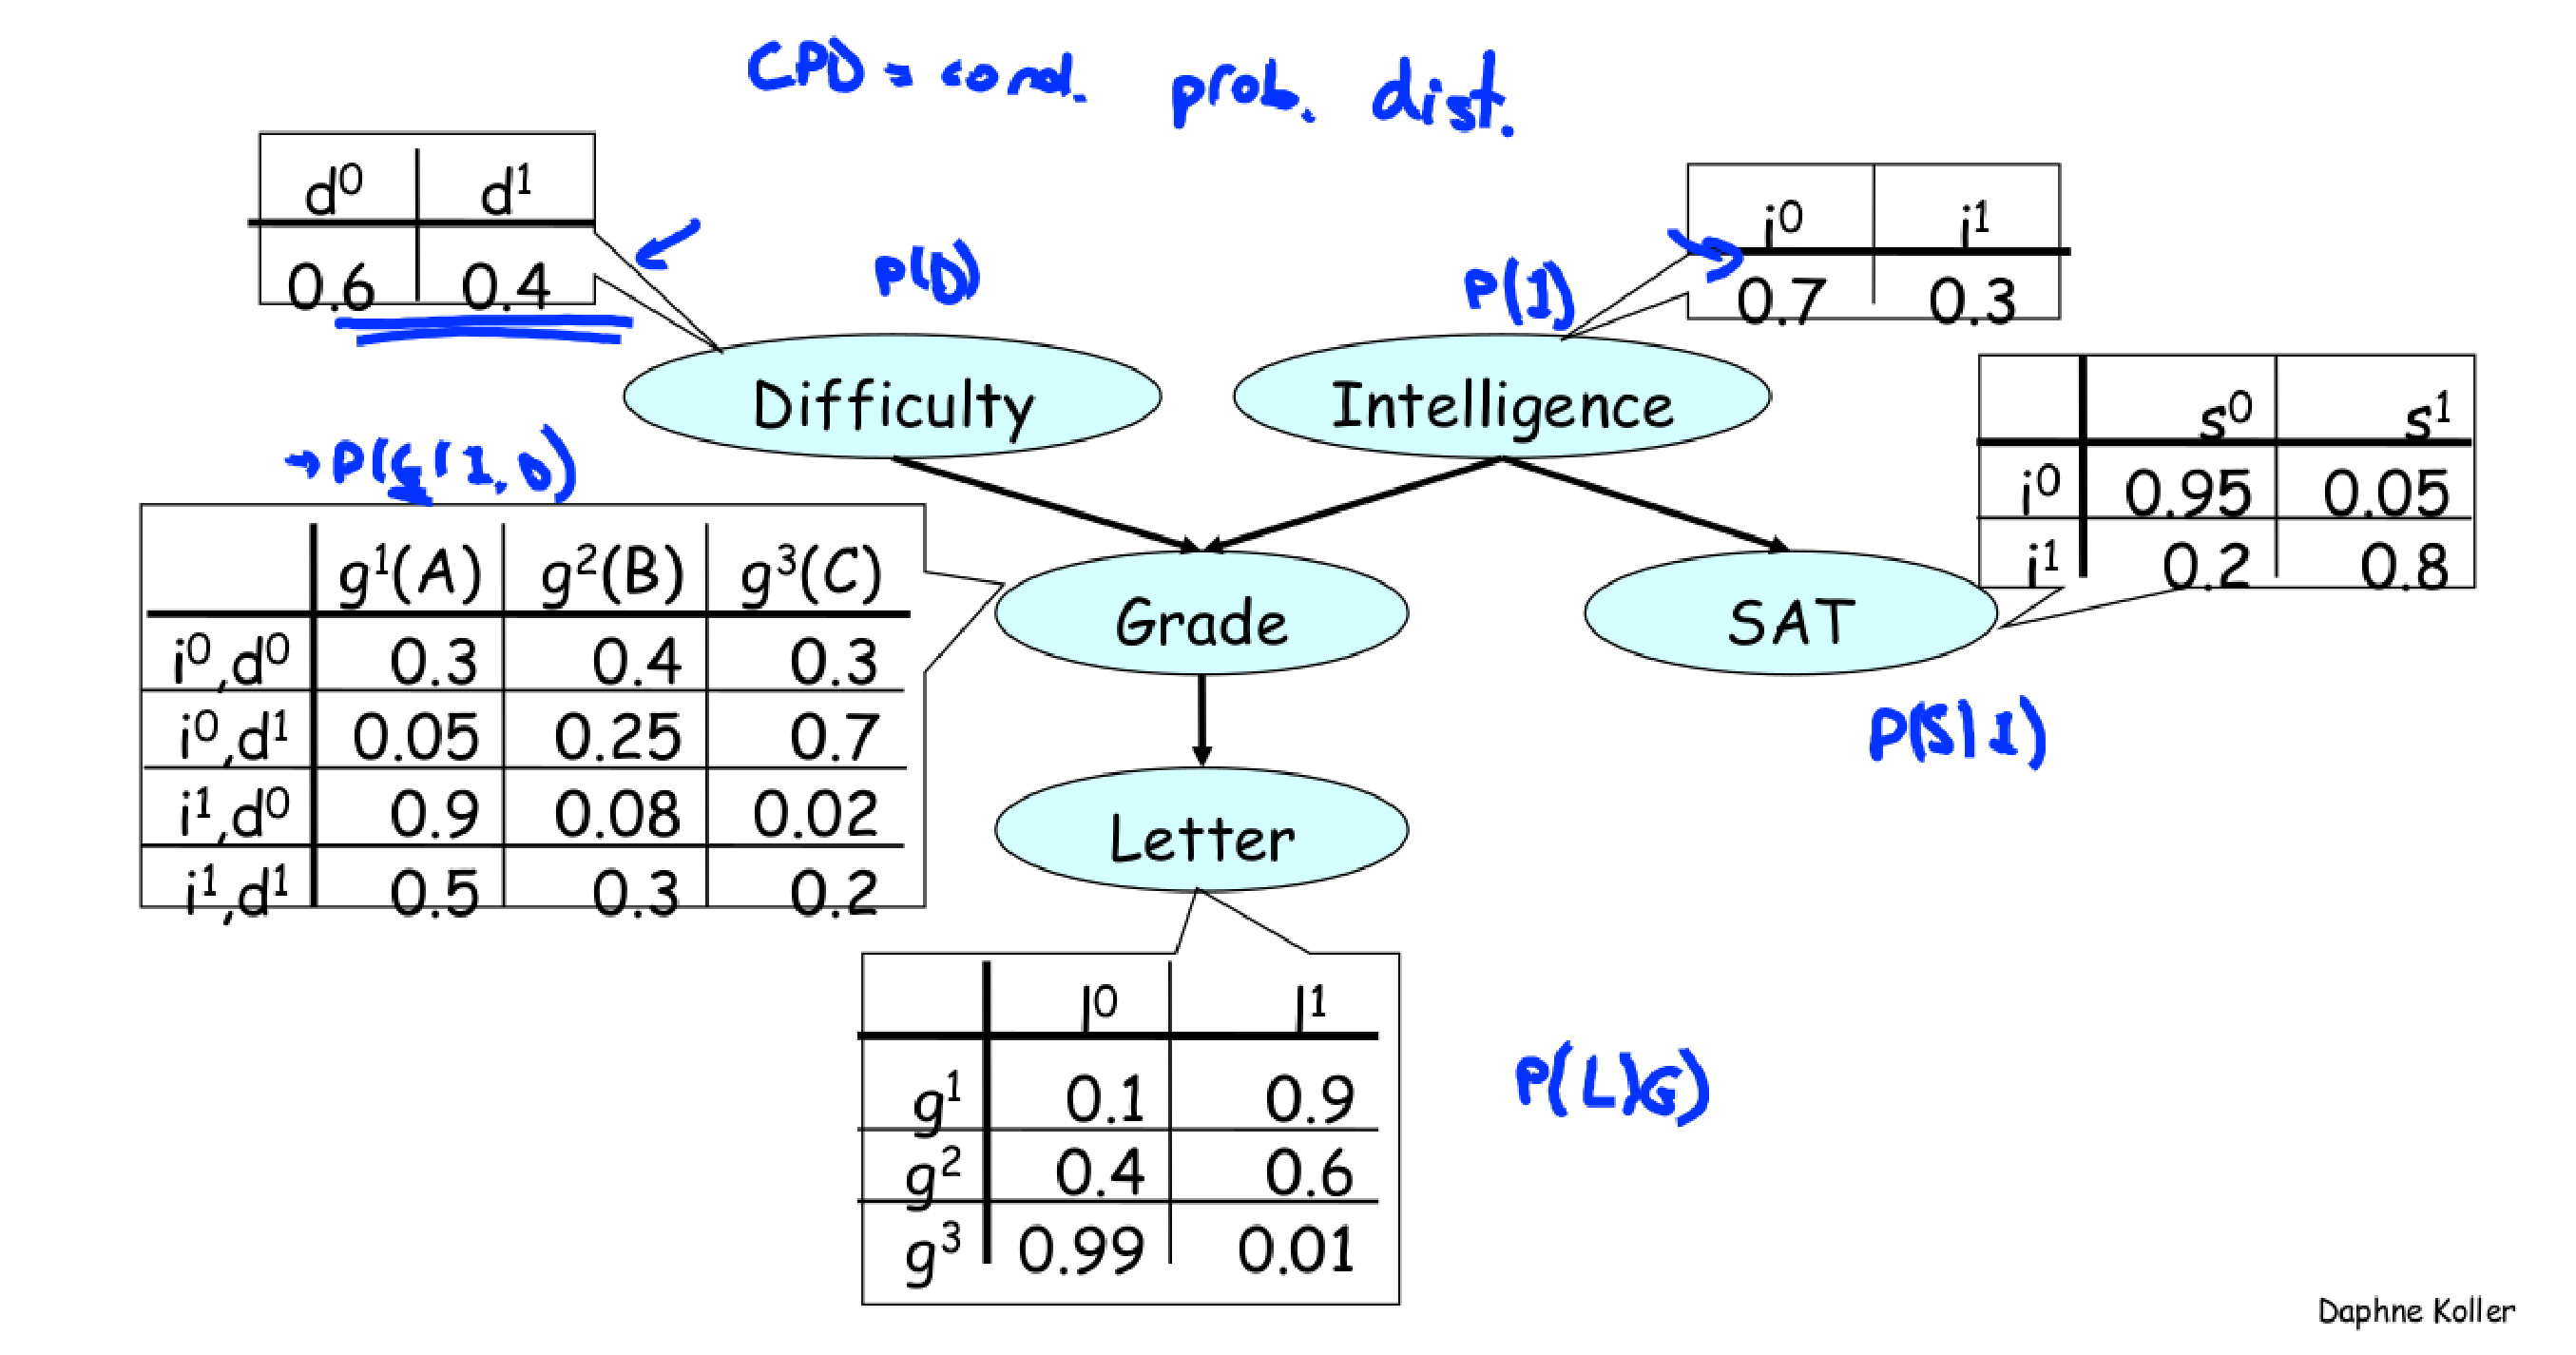
\includegraphics[scale = 0.3]{w1graphCPD}
\caption[Dependency Graph]{Dependency Graph: $D \rightarrow G$, $I \rightarrow G$, $I \rightarrow S$, $G \rightarrow L$}
\label{w1graphCPD}
\end{figure}


\subsection{Bayesian Network Definition}
Bayesian Network is:
\begin{itemize}
	\item a directed acyclic graph (DAG) G whose nodes represent the random variables $X_1,..,X_n$
	\item for each node $X_i$, there is a CPD: $P(X_i | Parents_G(X_i))$
	\item represents a joint distribution via the chain rule for Bayesian Networks in formula \ref{formChainRule} 
	\begin{align}\label{formChainRule}
	P(X_1,..,X_n) = \prod_i P(X_i|Parents_G(X_i))
	\end{align}
	\myaligns{Bayesian Network Definition}
\end{itemize}
We can prove that Bayesian Network is a legal distribution meaning it satisfies $P \geq 0$ and $\sum_i P(X_i) = 1$. The first one is trivial. The second one is proved as follow:
\begin{align*}
\sum_{D,I,G,S,L} P(D,I,G,S,L) 	&= \sum_{D,I,G,S,L} P(D)P(I)P(G|I,D)P(S|I)P(L|G) \\
								&= \sum_{D,I,G,S} P(D)P(I)P(G|I,D)P(S|I) \sum_L P(L|G) \\
								&= \sum_{D,I,G,S} P(D)P(I)P(G|I,D)P(S|I) * 1\\
								&= \sum_{D,I,G} P(D)P(I)P(G|I,D) \sum_S P(S|I)\\
								&= \sum_{D,I} P(D)P(I) \sum_G P(G|I,D)\\
								&= ...\\
								&= 1
\end{align*}

Another notation: Let G be a graph over $X_1, .., X_n$. A distribution $P$ is called to factorize over graph G if:
\begin{align*}
P(X_1, .., X_n) = \prod_i P(X_i | Par_G(X_i))
\end{align*}

\section{Reasoning Patterns}

\subsection{Causal Reasoning}
In a Bayesian network, if there is a path from one random variable to another, then the variable at the root of the path is said to affect the other random variables in the path via causal reasoning. For example, if $A \rightarrow B \rightarrow C$, then $A$ affects $B$ and $C$ via causal reasoning and $P(C)$ is generally \textbf{not equal} to $P(C|A)$.
Intuitively, inference goes in causal direction (direction of edges): \textbf{top down}.

\subsection{Evidential Reasoning}
In a Bayesian network, if there is a path from one random variable to another, then the variable at the end of the path is said to affect the other random variables in the path via evidential reasoning. For example, if $A \rightarrow B \rightarrow C$, then $C$ affects $A$ and $B$ via evidential reasoning and $P(A)$ is generally not equal to $P(A|C)$.
Bottom up: Condition the result, ask what the probability of the initial variables was (back from the cause), using Bayes' rule.

\subsection{Inter-causal Reasoning}
Flow of information between (for example) two causes of a single effect. When you condition the result, the causes are \textbf{no longer independent}. This also works across several edges and nodes. Don't really understand "explain away"! 


\chapter{Personal Note}
This is the week 1 of the course Probabilistic Graphical Models (pgm) by Prof. Daphne Koller hosted on Coursera. The week 1 covers quite a lot of notions from distribution to Bayesian Network.

\section{Distribution}
A probability distribution function (aka PDF, probability density function, probability function, or density) is a function that indicates the probability that a given random variable will take on a particular value. If a random variable is discrete (i.e. the value of the random variable is contained in a countable set of values), then the probability density function, $f(x)$ of a random variable $X$ is: $f(x) = P(X = x)$.

The multivariate form of a probability distribution function is the probability that a list of random variables will take on a list of values. If the random variables are discrete, the \textbf{joint probability density function}, $f(x_1, x_2, …, x_n)$ for random variables $X_1, X_2, ..., X_n$ is defined by: 
\begin{align}
f(x_1, x_2, \ldots, x_n) = P(X_1=x_1, X_2=x_2, \ldots, X_n=x_n)
\end{align}
\myaligns{Joint Distribution}

\section{Factors}
A factor is a function or a table or a mapping from every assignment of arguments to a real value. We define below factor $\Phi(X_1, \ldots, X_k)$ where $(X_1, \ldots, X_k)$ which is the scope (a set of random variables).
\begin{align}
\Phi: Val(X_1, \ldots, X_k) \rightarrow \mathbb{R}
\end{align}
\myaligns{Factor Definition}

\subsection{Examples of Factor}
Hence, according to the definition above, a joint distribution is a factor. Figure \ref{w1JointDistri} illustrates a joint distribution $P(I,D,G)$ where $I$, $D$, $G$ represents intelligence of a student $(0, 1)$, difficulty of a course $(0,1)$, and the final grade $(A,B,C)$ that student got from that course respectively.
\begin{figure}[!ht]
\centering
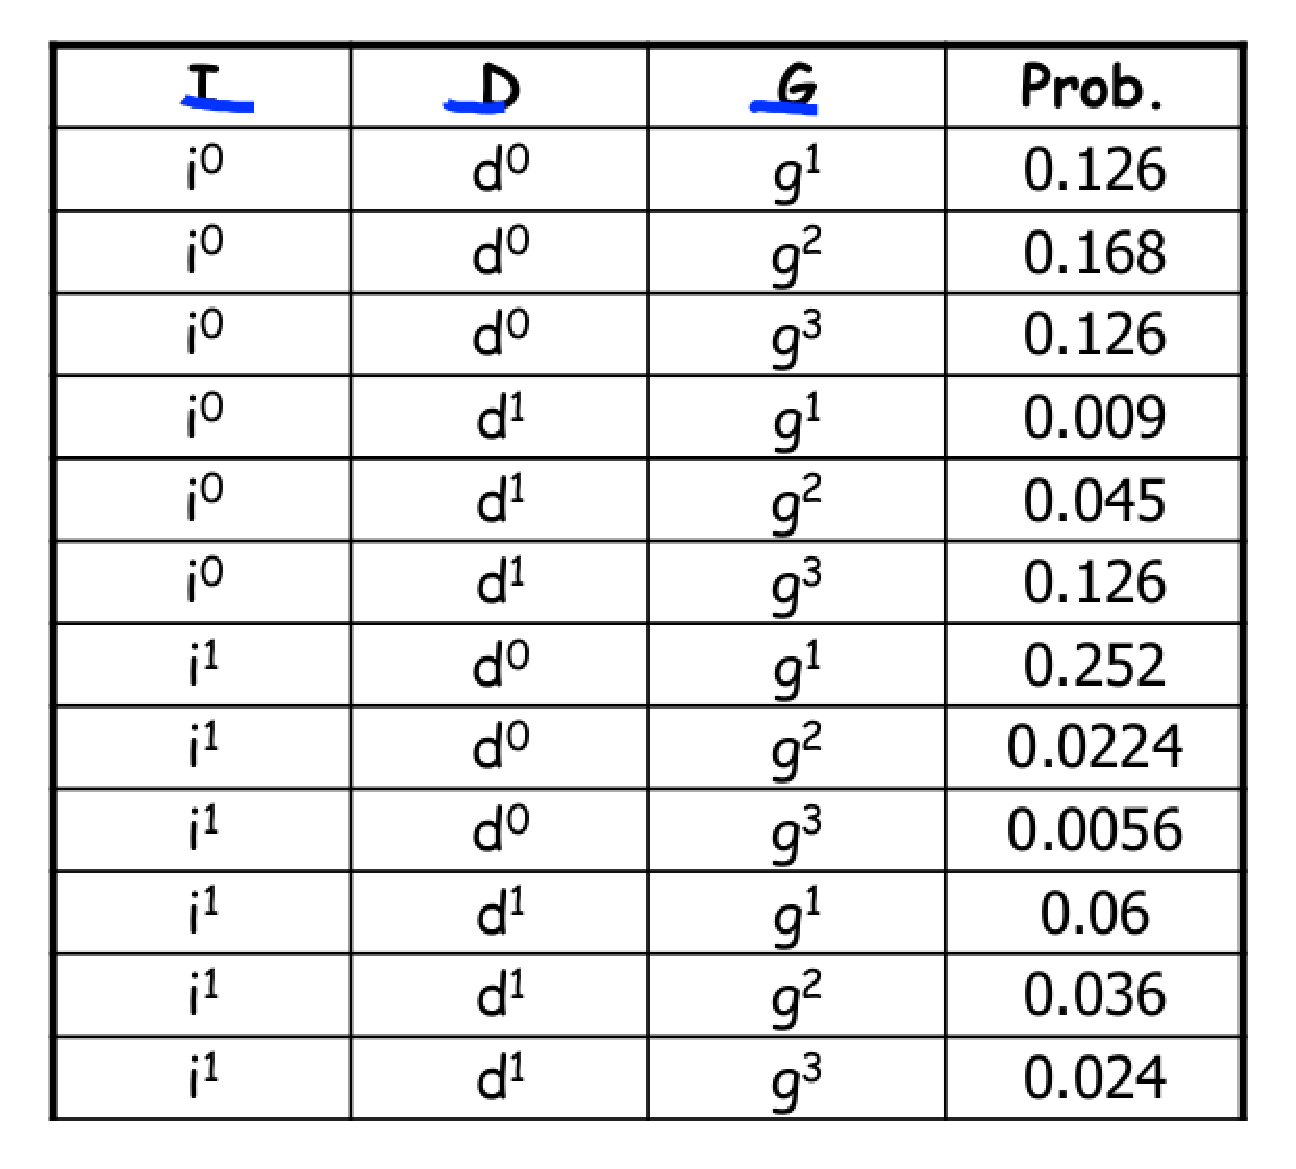
\includegraphics[scale = 0.3]{w1JointDistri}
\caption{Joint Distribution}
\label{w1JointDistri}
\end{figure}

Another example is UnnormaliCed Measure $P(I,D,g^1)$ which has scope $(I,D)$ because $G$ is always fixed to $g^1$. Another \textbf{important example} is Conditional Probability Distribution (CPD). Figure \ref{w1CPD} illustrates the \textbf{CPD} $P(G | I, D)$ which means for every combination of values to the variable $I$ and $D$, we have a probability distribution over $G$.  

\begin{figure}[!ht]
\centering
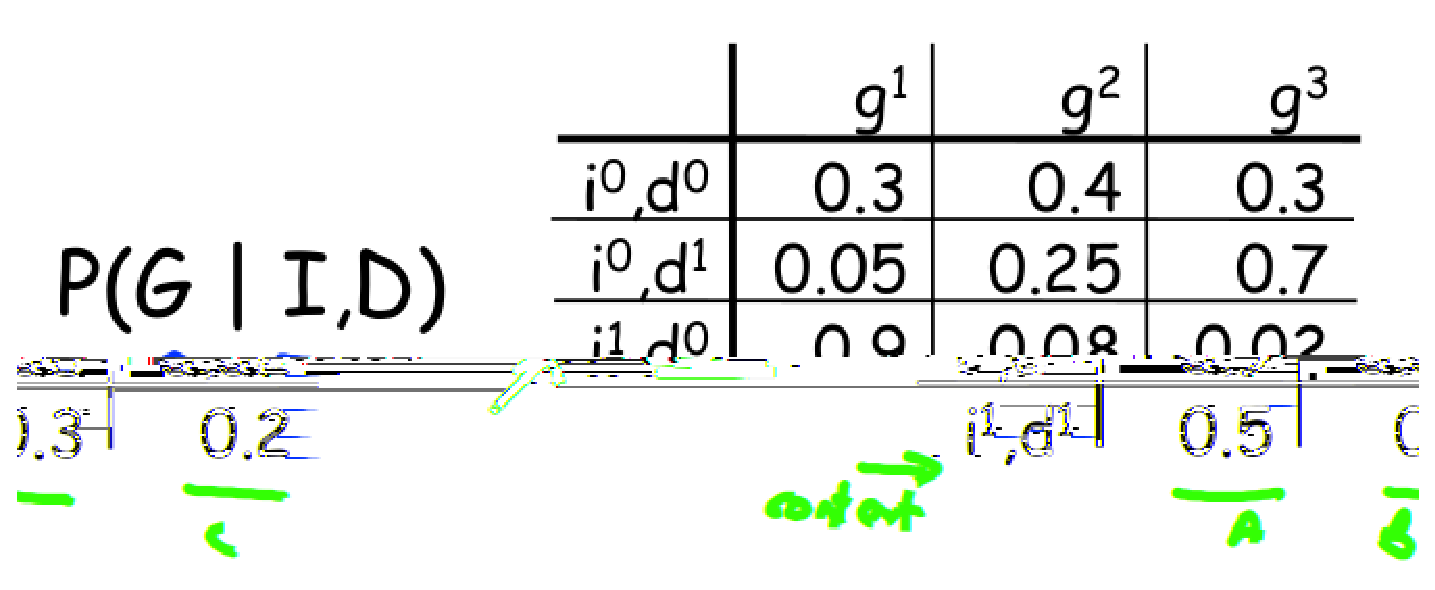
\includegraphics[scale = 0.4]{w1CPD}
\caption{Conditional Probability Distribution (CPD)}
\label{w1CPD}
\end{figure}

\section{Operations on Factors}
\subsection{Factor Products}
If $\Phi_1(A,B)$ and $\Phi_2(B,C)$ are two factors then we compute their product of $\Phi(A,B,C)$ by multiplying $\Phi_1(A,B)\Phi_2(B,C)$ for all common values of $B$ (see figure \ref{w1FactProd}).

\begin{figure}[!ht]
\centering
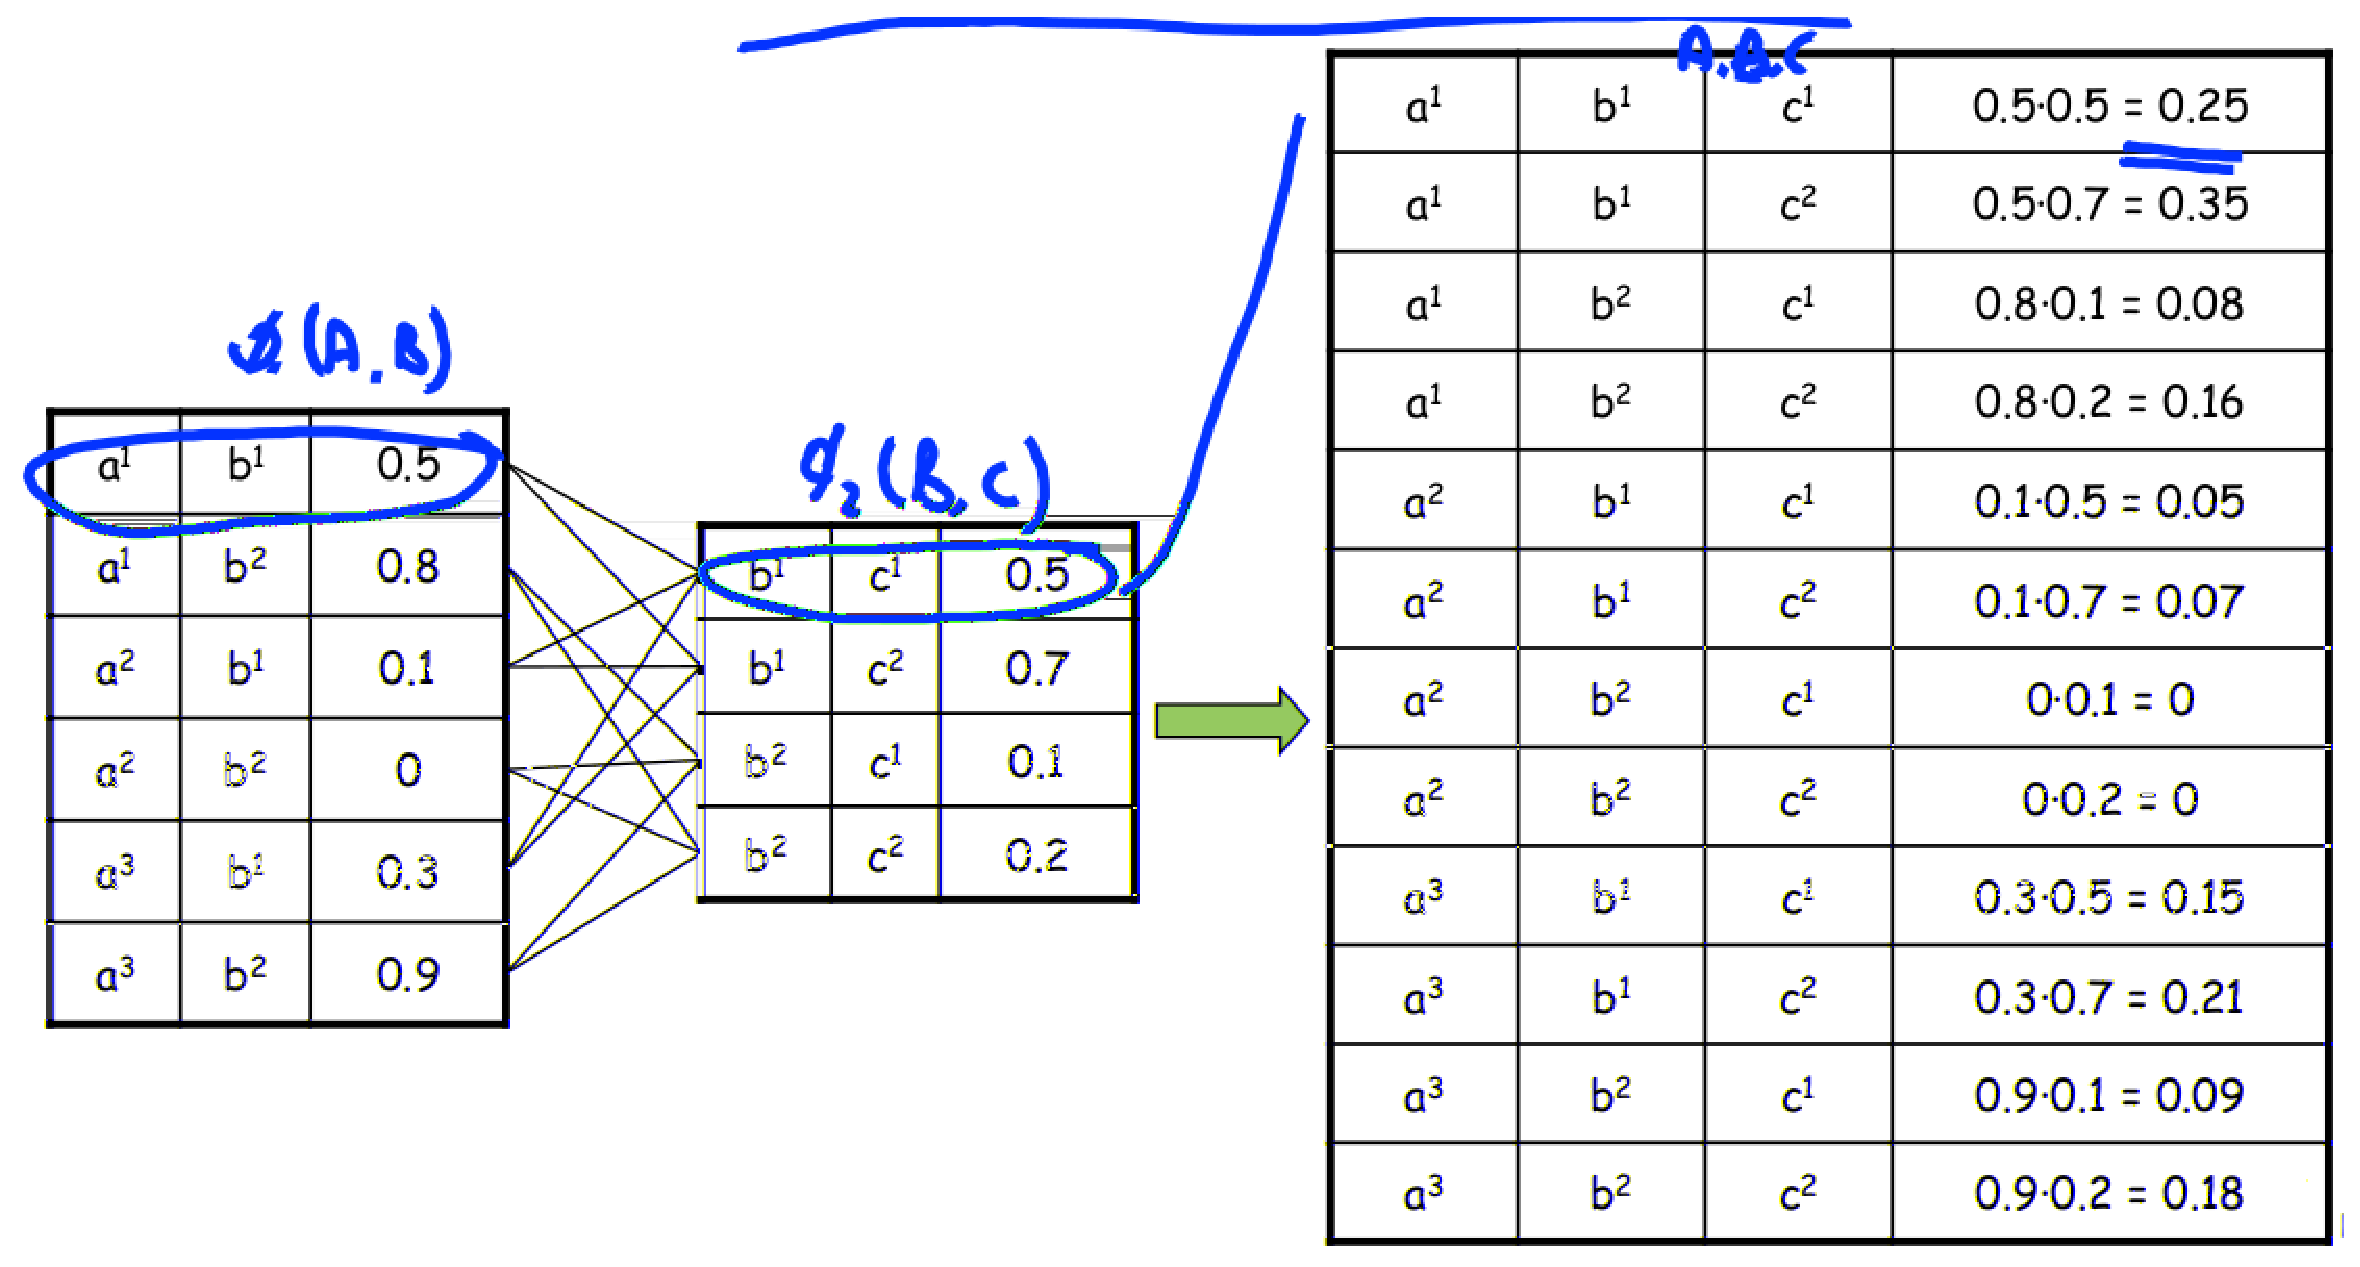
\includegraphics[scale = 0.3]{w1FactProd}
\caption{Factor Products}
\label{w1FactProd}
\end{figure}

\subsection{Factor Marginalization}
That's when we want to reduce the scope. For example, we reduce scope $(A,B,C)$ to $(A,C)$ by summing over $B$ for every assignment of $(A,C)$ (figure \ref{w1FactMarginal}).

\begin{figure}[!ht]
\centering
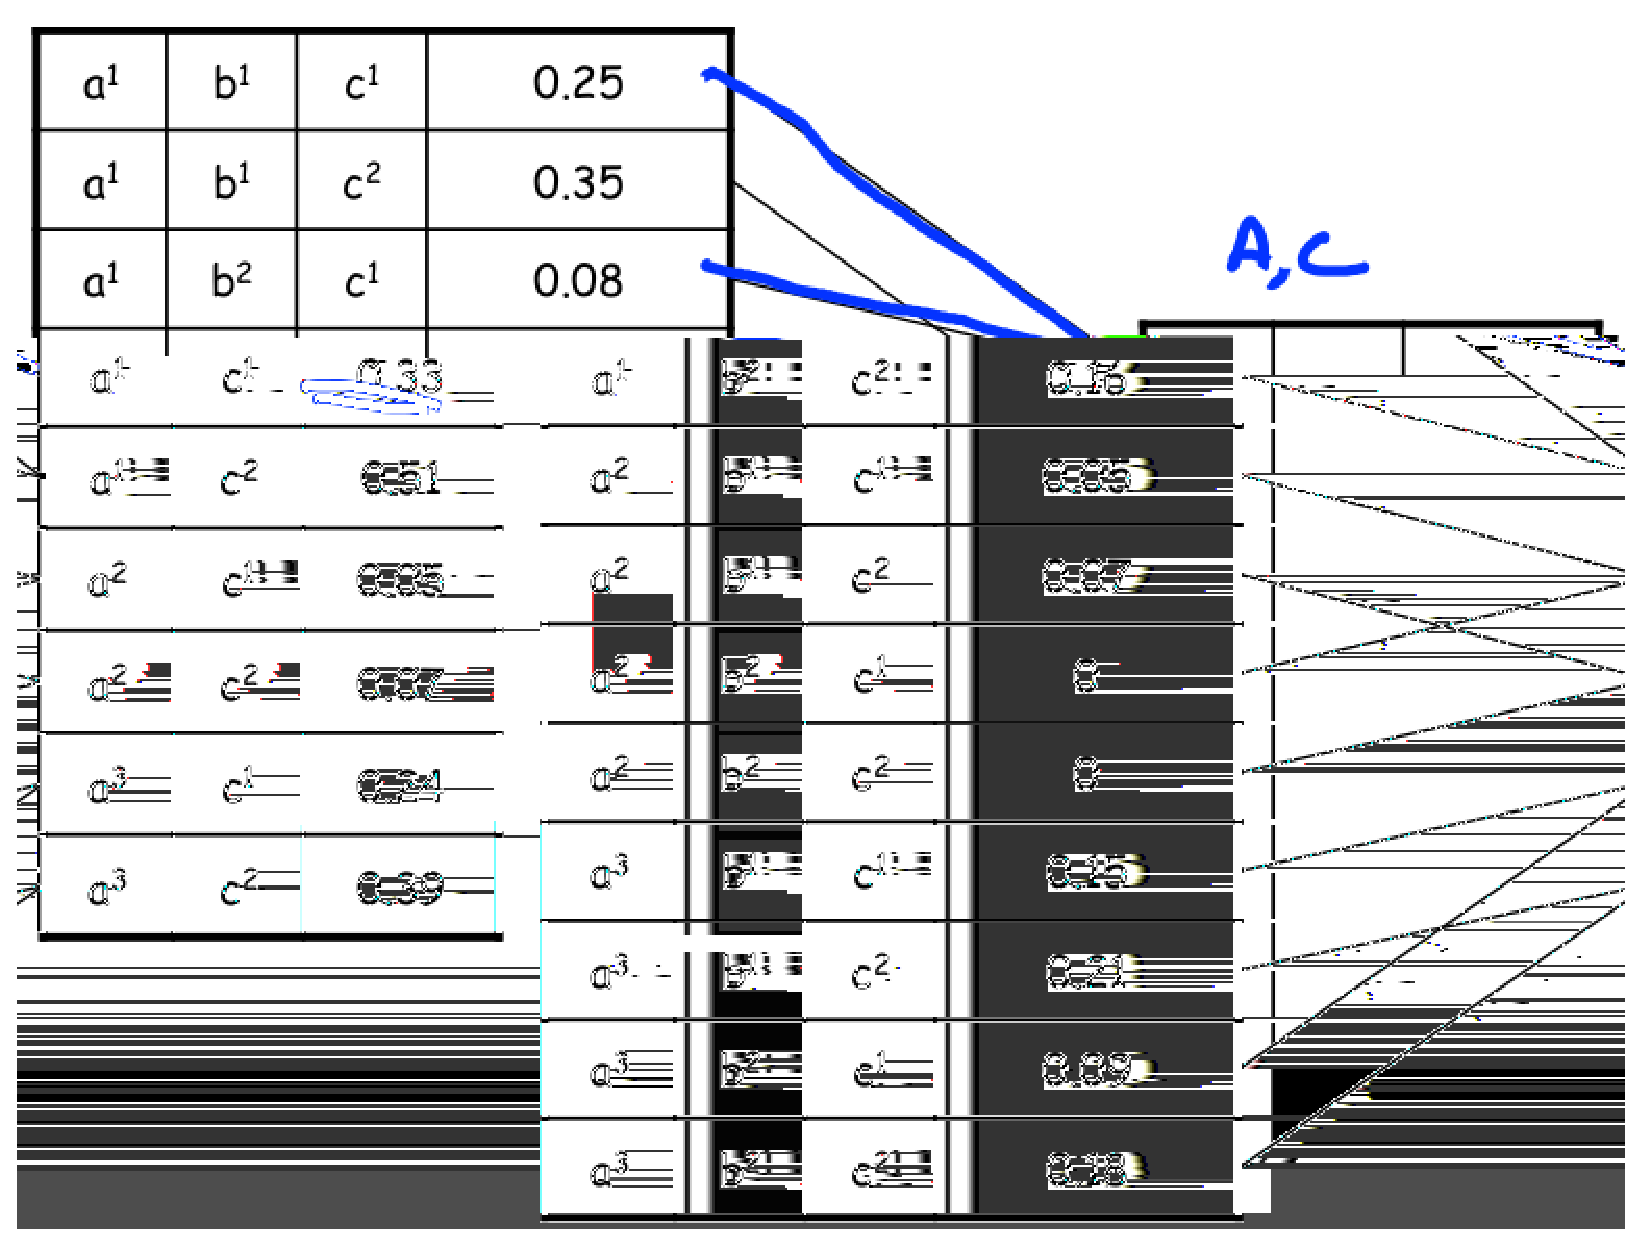
\includegraphics[scale = 0.35]{w1FactMarginal}
\caption{Factor Marginalization}
\label{w1FactMarginal}
\end{figure}

\subsection{Factor Reduction}
That's when we fix a random variable in the scope by one value (in its set of values). For example, $\Phi(A,B,C)$ is reduced to $\Phi(A,B | C = c^1)$ in illustration \ref{w1FactReduce}.
\begin{figure}[!ht]
\centering
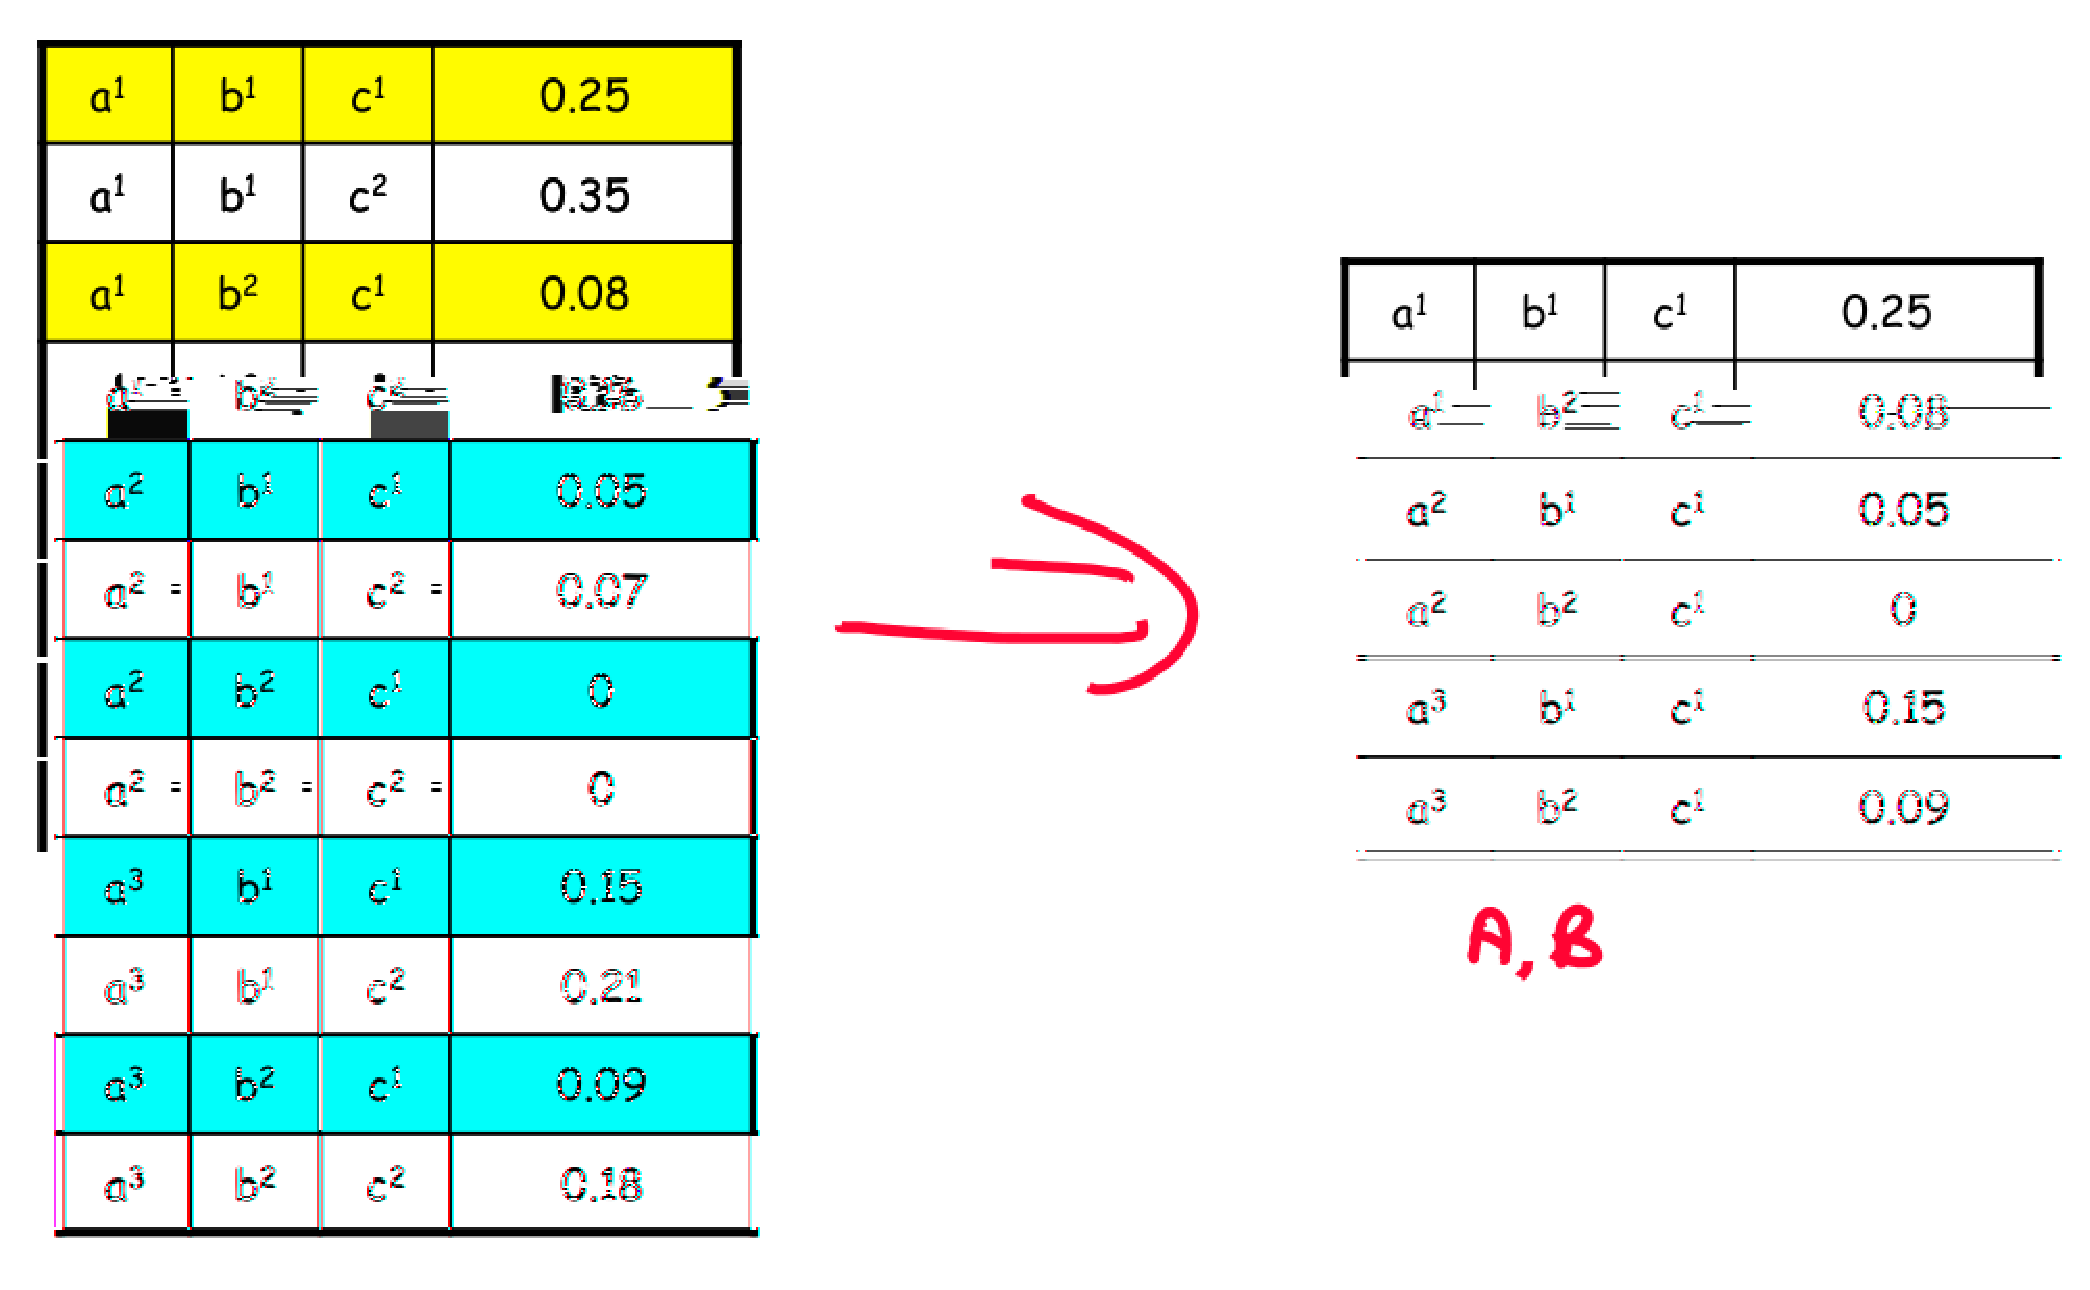
\includegraphics[scale = 0.35]{w1FactReduce}
\caption{Factor Reduction}
\label{w1FactReduce}
\end{figure}

\section{Semantics And Factorization}
\subsection{The Student Example}
The student example involving the situation where students take a course. It contains the following random variables:
\begin{itemize}
	\item Course \textbf{D}ifficulty $(D)$ ($0$ = not difficult, $1$ = difficult)
	\item Student \textbf{I}ntelligence $(I)$ ($0$ = not intelligent, $1$ = intelligent)
	\item \textbf{G}rade $(G)$ ($1$ = A, $2$ = B, $3$ = C)
	\item Student \textbf{S}AT score $(S)$ ($0$ = not good, $1$ = good)
	\item Reference \textbf{L}etter from the prof. of this course $(L)$ ($0$ = not referred, $1$ = referred)
\end{itemize}

The dependency graph is shown in figure \ref{w1graphCPD}. Intuitively, we can see the directed edge meaning a strong relation between the 2 variables. We also annotate each node of the dependency graph to a CPD (Conditional Probability Distribution). NB: I do not know where this comes from, maybe we can calculate them from the data set. We have the chain rule for Bayesian Networks in this example is described in formula below.
\begin{align}
P(G|I,D)P(S|I)P(L|G)P(D)P(I) = P(D,I,G,S,L)
\end{align}
\myaligns{Chain Rule for Bayesian Networks}

\begin{figure}[!ht]
\centering
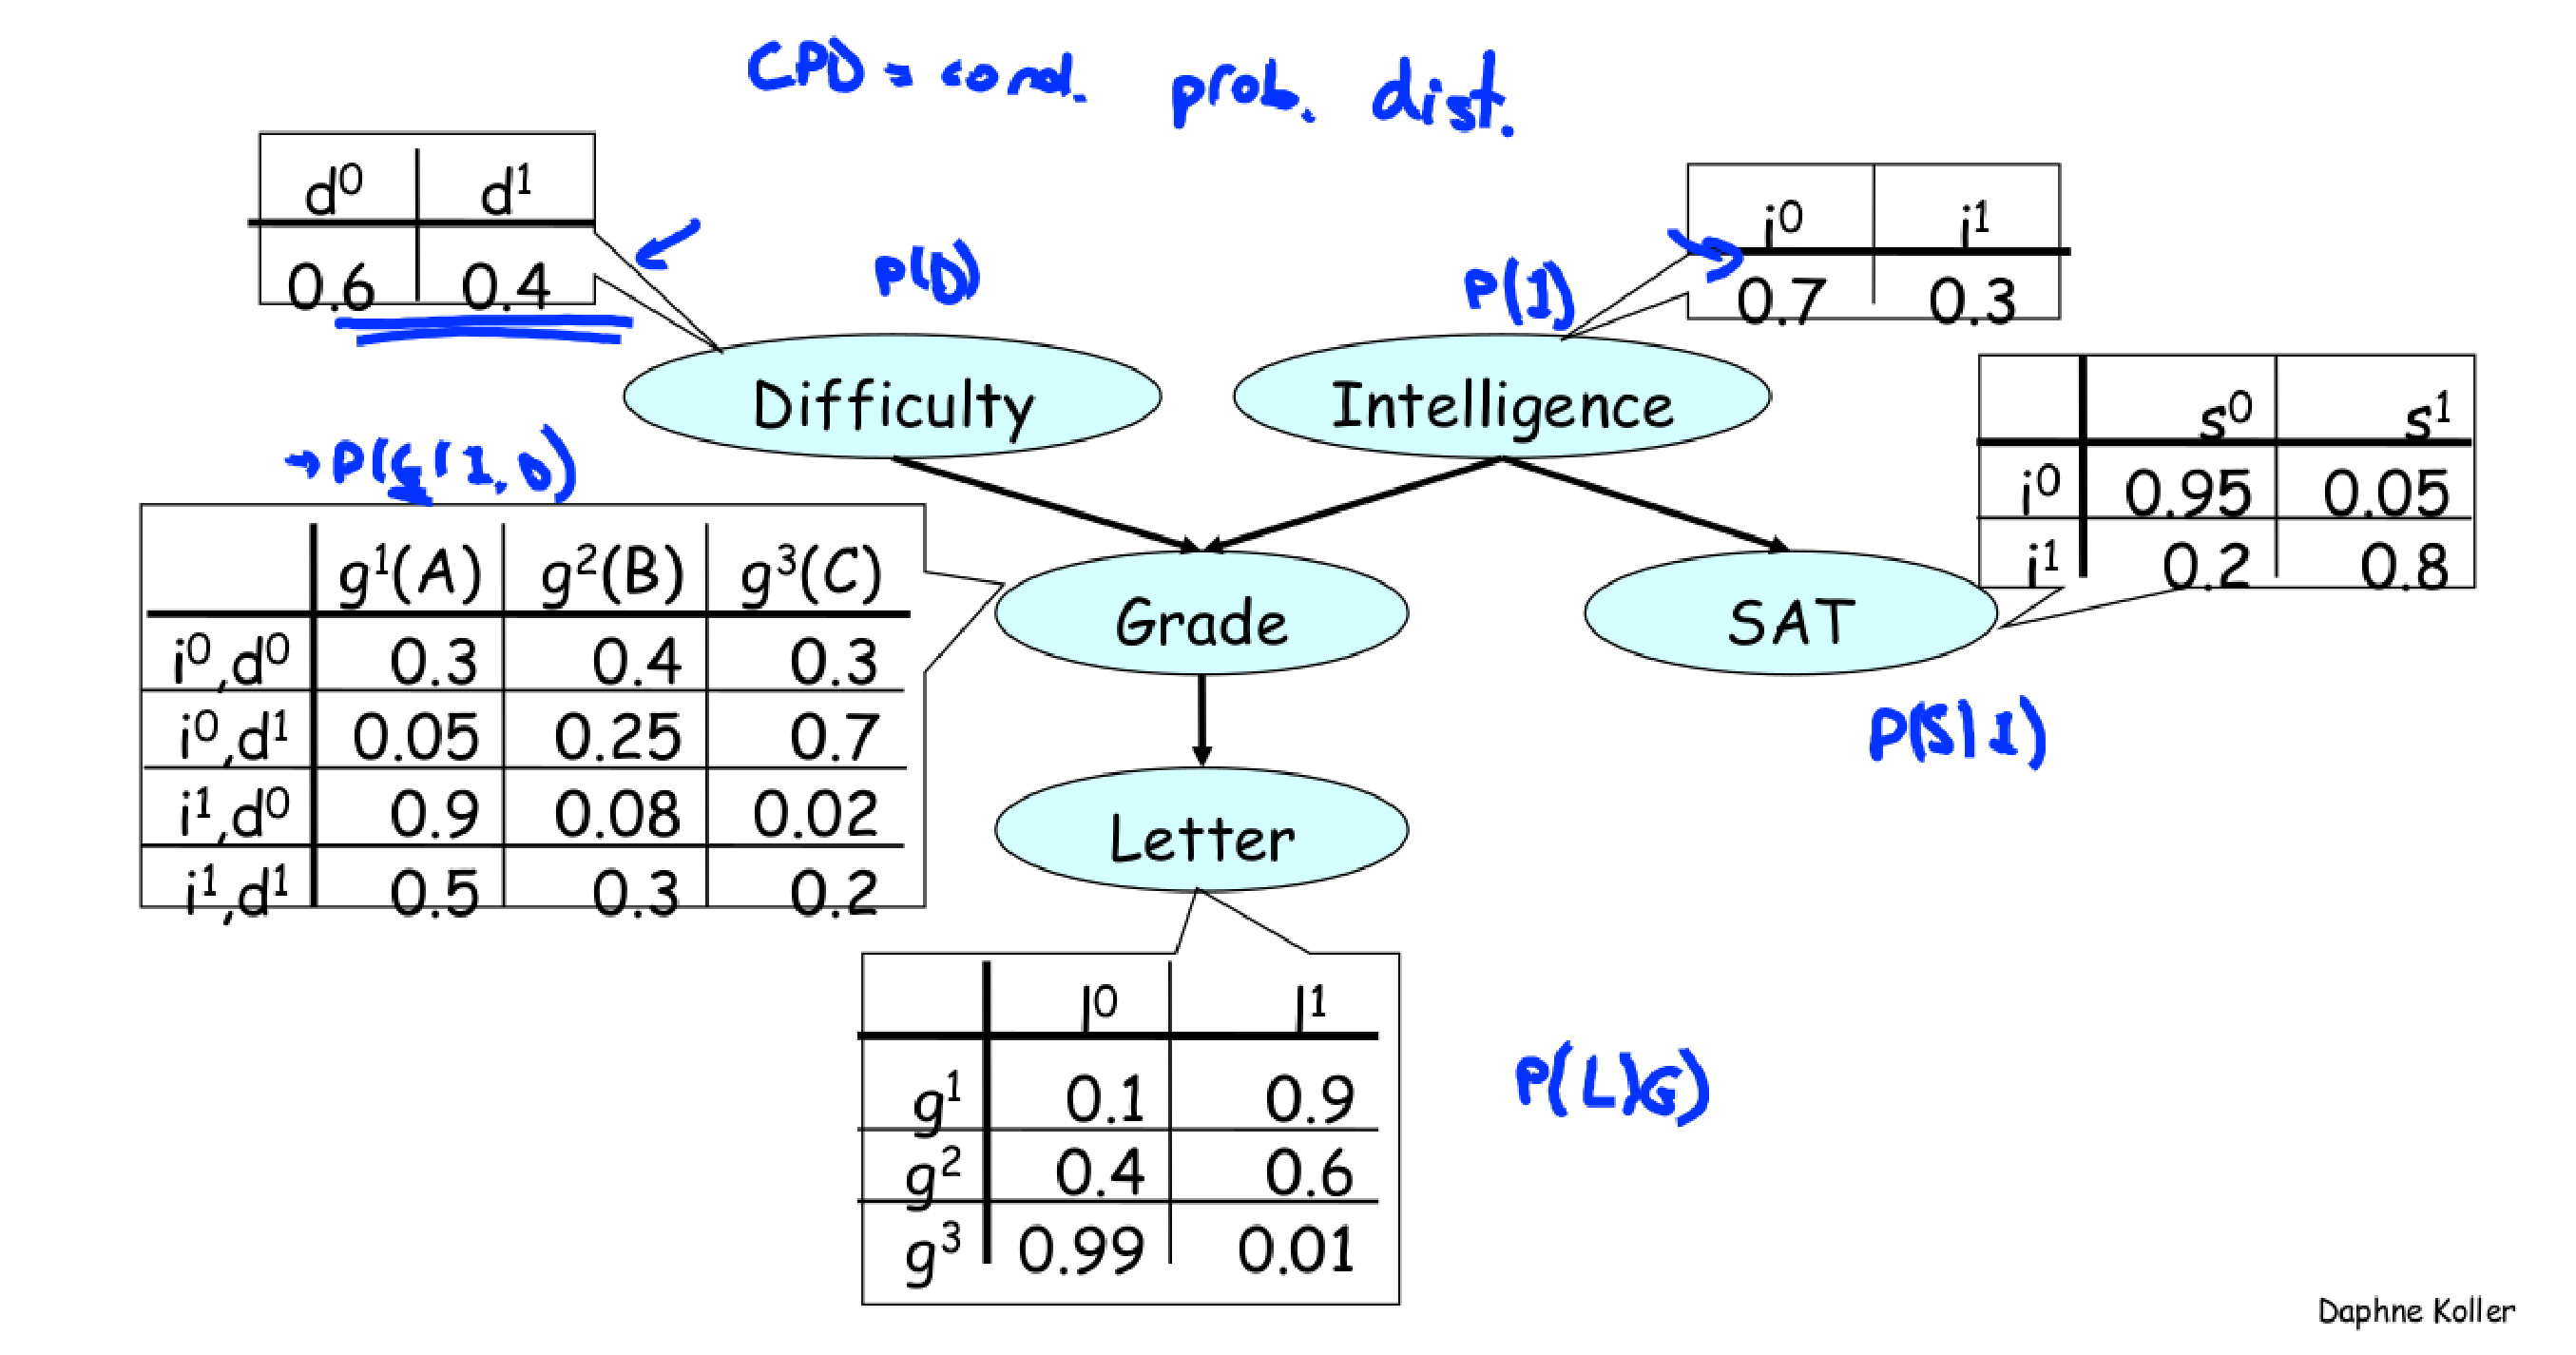
\includegraphics[scale = 0.3]{w1graphCPD}
\caption[Dependency Graph]{Dependency Graph: $D \rightarrow G$, $I \rightarrow G$, $I \rightarrow S$, $G \rightarrow L$}
\label{w1graphCPD}
\end{figure}


\subsection{Bayesian Network Definition}
Bayesian Network is:
\begin{itemize}
	\item a directed acyclic graph (DAG) G whose nodes represent the random variables $X_1,..,X_n$
	\item for each node $X_i$, there is a CPD: $P(X_i | Parents_G(X_i))$
	\item represents a joint distribution via the chain rule for Bayesian Networks in formula \ref{formChainRule} 
	\begin{align}\label{formChainRule}
	P(X_1,..,X_n) = \prod_i P(X_i|Parents_G(X_i))
	\end{align}
	\myaligns{Bayesian Network Definition}
\end{itemize}
We can prove that Bayesian Network is a legal distribution meaning it satisfies $P \geq 0$ and $\sum_i P(X_i) = 1$. The first one is trivial. The second one is proved as follow:
\begin{align*}
\sum_{D,I,G,S,L} P(D,I,G,S,L) 	&= \sum_{D,I,G,S,L} P(D)P(I)P(G|I,D)P(S|I)P(L|G) \\
								&= \sum_{D,I,G,S} P(D)P(I)P(G|I,D)P(S|I) \sum_L P(L|G) \\
								&= \sum_{D,I,G,S} P(D)P(I)P(G|I,D)P(S|I) * 1\\
								&= \sum_{D,I,G} P(D)P(I)P(G|I,D) \sum_S P(S|I)\\
								&= \sum_{D,I} P(D)P(I) \sum_G P(G|I,D)\\
								&= ...\\
								&= 1
\end{align*}

Another notation: Let G be a graph over $X_1, .., X_n$. A distribution $P$ is called to factorize over graph G if:
\begin{align*}
P(X_1, .., X_n) = \prod_i P(X_i | Par_G(X_i))
\end{align*}

\section{Reasoning Patterns}

\subsection{Causal Reasoning}
In a Bayesian network, if there is a path from one random variable to another, then the variable at the root of the path is said to affect the other random variables in the path via causal reasoning. For example, if $A \rightarrow B \rightarrow C$, then $A$ affects $B$ and $C$ via causal reasoning and $P(C)$ is generally \textbf{not equal} to $P(C|A)$.
Intuitively, inference goes in causal direction (direction of edges): \textbf{top down}.

\subsection{Evidential Reasoning}
In a Bayesian network, if there is a path from one random variable to another, then the variable at the end of the path is said to affect the other random variables in the path via evidential reasoning. For example, if $A \rightarrow B \rightarrow C$, then $C$ affects $A$ and $B$ via evidential reasoning and $P(A)$ is generally not equal to $P(A|C)$.
Bottom up: Condition the result, ask what the probability of the initial variables was (back from the cause), using Bayes' rule.

\subsection{Inter-causal Reasoning}
Flow of information between (for example) two causes of a single effect. When you condition the result, the causes are \textbf{no longer independent}. This also works across several edges and nodes. Don't really understand "explain away"! 


%\printindex
\end{document}
